\documentclass[../the.tex]{subfiles}

\begin{document}

{\fontsize{13}{12} \selectfont
Chương này sẽ trình bày các nghiên cứu có liên quan, khái niệm về thị giác máy tính, mô hình nơ-ron tích chập, lý thuyết về các mô hình phát hiện đối tượng và phương pháp đánh giá mô hình.
}

\section{Các nghiên cứu liên quan}
\label{sec:nnlq}
{\fontsize{13}{12} \selectfont

	Yang và Thung \cite{yang2016classification} đã so sánh mô hình Support Vector Model (SVM) với
	mô hình mạng nơ-ron tích chập (CNN) dựa trên tập dữ liệu khoảng 2400 hình
	ảnh và phân ra làm 6 lớp: thủy tinh, giấy, kim loại, nhựa, bìa cứng, và các loại
	rác khác. Nhóm nghiên cứu đã sử dụng tăng cường dữ liệu bằng việc xoay, điều chỉnh độ sáng,
	dịch chuyển và cắt các hình ảnh một cách ngẫu nhiên. Sau đó nhóm huấn luyện mô hình và đạt kết quả 67\% cho SVM và 22\% cho CNN.
	Tuy kết quả của nhóm tác giả không đạt mong muốn như kì vọng nhưng bộ dữ liệu TrashNet sau này của nhóm đã được sử dụng rộng rãi cho các nghiên cứu tương tự.
}

\bigskip

{\fontsize{13}{12} \selectfont

	Ngoài ra, Jash và Sagar \cite{shah2022method} đã đề xuất một mô hình CNN dựa trên 25.077
	hình ảnh chia làm 2 lớp: rác hữu cơ và rác tái chế. Mô hình nhận ảnh đầu vào là
	hình có kích thước 224x224 với mã màu RGB, gồm 6 lớp tích chập, 3 lớp tổng
	hợp, và 3 lớp kết nối. ReLU sẽ là hàm kích hoạt. Đầu ra của mô hình là nơ-ron
	có giá trị 0 (rác hữu cơ) và 1 (rác tái chế). Nhóm nghiên cứu so sánh kết quả
	của mô hình tự xây dựng với VGG16 \cite{simonyan2014very} và ResNet-34.
	Mô hình đạt độ chính xác lên đến 0.9496.
}

\bigskip

{\fontsize{13}{12} \selectfont

	Ahmad và ctv. \cite{ahmad2020intelligent} đã áp dụng các phương pháp kết hợp sớm, kết hợp muộn
	và kết hợp kép các mô hình học sâu trên tập dự liệu 2.527 hình ảnh đưuọc cung cấp bởi Kaggle, tậo dữ liệu
	được chia làm 6 lớp giống như nghiên cứu của Yang và Thung \cite{yang2016classification}. Trong nghiên cứu này,
	nhóm tác giả đạt kết quả cao và đưa ra kết luận có thể đạt được hiệu suất phân
	loại chất thải tốt hơn bằng cách kết hợp tối ưu các mô hình học sâu thông qua
	các phương pháp thích hợp. Tuy nhiên nhóm nghiên cứu cũng đang mở rộng
	quy mô dữ liệu trong tương lai.
}

\bigskip

{\fontsize{13}{12} \selectfont

	Ở Việt Nam, nhóm nghiên cứu đến từ Đại học Quốc gia Hà Nội, cục Viễn
	Thám Quốc gia và viện Khoa học Đo đạc và Bản Đồ thuộc Bộ Tài Nguyên và
	Môi Trường \cite{nhung2021nghien} đã sử dụng mô hình mạng nơ-ron tích chập sâu (DCNN) được
	huấn luyện và thử nghiệm trên 95 hình ảnh được chụp từ máy bay không người
	lái (UAV) Phantom 4 Pro ở khu vực ven biển Hội An (Quảng Nam). Mô hình
	đạt độ chính xác trong việc phân loại hình ảnh rác thải nhựa ven biển là 87\%.
	Các nghiên cứu trên là tiêu biểu của việc ứng dụng công nghệ phát hiện
	và phân loại rác thải.
}
\bigskip

{\fontsize{13}{12} \selectfont

	Đối với các nghiên cứu về phân loại hoặc phân đoạn rác thải có nhóm nghiên cứu của tác giả Pedro F. Proença \cite{proença2020taco} cung cấp bộ dữ liệu Taco với đa dạng nhãn về các loại rác.
	Nhóm nghiên cứu sử dụng mô hình Mask R-CNN để huấn luyện và đạt được kết quả 17.6\% với khả năng phát hiện và phân loại, 26.2\% với với khả năng chỉ phát hiện rác.
	Vì độ đa dạng của đối tượng cũng như hình nền, mô hình của nhóm tác giả dễ bị phát hiện nhầm giữa đối tượng và nền hoặc bỏ sót đi các vật thể nhỏ. Tuy vậy, nhóm tác giả cũng tin tưởng rằng bộ dữ liệu sẽ mang vấn đề tích cực và mong cộng đồng cùng chung tay xây dựng tập dữ liệu tốt hơn.
}
\bigskip

{\fontsize{13}{12} \selectfont

	Sylwia Majchrowska \cite{Majchrowska_2022} áp dụng việc kết hợp các bộ dữ liệu về rác để huấn luyện mô hình theo bảy lớp theo tình hình ở Pomerania, Ba Lan và đạt kết quả 66.4\% với phát hiện một lớp.
	Đề tài nghiên cứu sẽ áp dụng ý tưởng của \cite{Majchrowska_2022} và dữ liệu của \cite{yang2016classification}, \cite{proença2020taco} để thực hiện.
}
\section{Thị giác máy tính}
\label{sec:ttmt}

{\fontsize{13}{12}\selectfont
Thị giác máy tính là một trong những lĩnh vực quan trọng của khoa học máy tính và trí tuệ nhân tạo. Thị giác máy tính là một công nghệ giúp tự động nhân biết và mô tả hình ảnh một các chính xác và hiệu quả.
Hình \ref{fig:computer_vision} giải thích quá trình con người ghi lại hình ảnh đối tượng thông qua võng mạc của mắt,
sau đó bộ não tiếp nhận và nhận dạng ra đối tượng. Một người có thể dễ dàng nhận biết và phát hiện đối tượng trong bức ảnh một các chính xác vị trí của chúng.
Tuy nhiên việc này lại khó khăn với máy tính, hệ thống phải
tiếp nhận hình ảnh thông qua thiết bị ghi hình, "đọc" và "hiểu" hình ảnh dưới dạng ma trận số của tập hợp các điểm ảnh,
sau đó được mô hình huấn luyện từ trước để nhận dạng các đối tượng trong ảnh.
Tuy vẫn chưa thể chính xác được như thị giác của con người nhưng đã có rất nhiều ứng dụng hữu ích, điểm hình như điểm danh bằng khuôn mặt, phát hiện các bệnh bằng chuẩn đoán hình ảnh, công nghệ xe tự hành.
{\fontsize{13}{12} \selectfont
\begin{figure}[H]
	\centering
	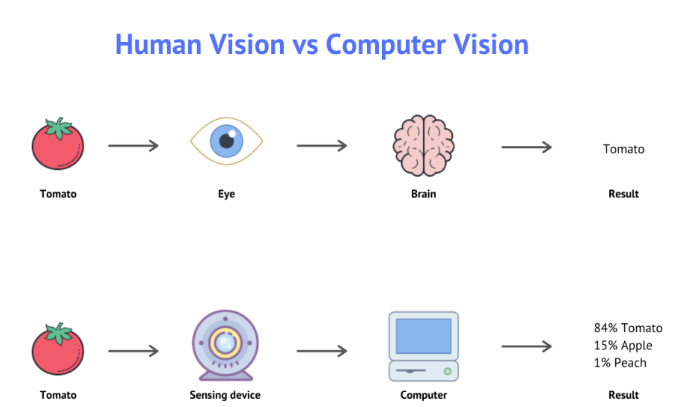
\includegraphics[width=1\textwidth]{computer_vision.PNG}
	\caption{Hệ thống thị giác của con người và máy tính}
	\label{fig:computer_vision}
\end{figure}}
Năm 1966, dự án mang tên "Summer Vision Project" \cite{Papert1966TheSV} của Seymour Papert và Marvin Minsky  đã mở đầu cho việc nghiên cứu về thị giác máy tính sau khi nỗ lực trong hai tháng để tạo ra một hệ thống máy tính có thể
nhận dạng các vật thể trong ảnh. Từ đó đến nay, thị giác máy tính đã phát triển vượt bậc để thực hiện được những tác vụ phổ biến như:

{\fontsize{13}{12} \selectfont
\begin{itemize}
	\item Phân loại hình ảnh: Phân loại hình ảnh cho phép máy tính quan sát và phân loại chính xác một hình ảnh thuộc loại nào.
	      Ví dụ là camera có thể nhận diện khuôn mặt trong ảnh.
	\item Phát hiện đối tượng: Xác định và phân loại các vật thể khác nhau trong hình ảnh hoặc video bằng ô bao quanh đối tượng (Bbox). Ví dụ phát hiện cây cối hay con người.
	\item Theo dõi đối tượng: Theo dõi đối tượng sử dụng mô hình học sâu để xác định và theo dõi các mục tiêu. Ví dụ giám sát giao thông tại cái điểm có đèn giao thông.
	\item Phân đoạn: Xác định đối tượng bằng cách chia nhỏ đối tượng thành các vùng khác nhau dựa trên các điểm ảnh quan sát được. Khác với nhận dạng đối tượng, phân đoạn sẽ xác định hình dạng cụ thể của đối tượng.
	\item Truy xuất hình ảnh dựa trên nội dung: có khả năng tìm kiếm các hình ảnh kỹ thuật số cụ thể trong cơ sở dữ liệu lớn.
\end{itemize}
}
\bigskip

Mạng nơ-ron truyền thống (Neural Network) hoạt động không thực sự hiệu quả với dữ liệu đầu vào là hình ảnh vì các pixel liền kề có sự phụ thuộc lẫn nhau.
việc biến đổi thành vector sẽ mất đi tính phụ thuộc, thay đổi ý nghĩa hình ảnh hoặc đòi hỏi dữ liệu lớn để huấn luyện.

}

\section{Mạng nơ-ron tích chập }
\label{sec:cnn}
{\fontsize{13}{12} \selectfont
	Mạng nơ-ron tích chập (CNN) là mạng no-ron phổ biến sử dụng cho dữ liệu ảnh.
	CNN được thiết kế để tự động học các đặc trưng từ dữ liệu hình ảnh thông qua các tầng tích chập, lần đầu được lấy cảm hứng từ một nghiên cứ năm 1959 của Hubel \& Wiesel \cite{hubel1962receptive} thông qua phản ứng của các tế bào thần kinh trên não mèo. Với sự kết hợp phát triển đồng bộ và mãnh mẽ của khả năng tính toán của máy tính cùng các phương pháp tối ưu,
	sau gần 20 năm nghiên cứu, CNN hiện đã và đang phát triển rất nhiều kiến trúc mạng khác nhau. Bắt đầu từ năm 1998 với lần đầu tiên sử dụng mạng tích chập trong tác vụ phân loại chữ số viết tay của Yan Lecun
	\cite{lecun1998gradient} cho đến thành công đầu tiên của mạng AlexNet khi vượt qua được các phương pháp đặc trưng truyền thống như HOG, SHIFT vào năm 2012. Sau đó các mạng mới lần lượt như VGG Net, GoogleNet, ResNet, DenseNet,\dots
	đã rút gọn quá trình huấn luyện từ vài ngày xuống còn vài giờ và tăng độ chính xác của mô hình.

	Cấu trúc cơ bản của CNN gồm lớp tích chập, hàm kích hoạt, lớp gộp và lớp kết nối đầy đủ, được thay đổi về số lượng và cách sắp xếp để tạo ra các mô hình huấn luyện phù hợp cho từng bài toán khác nhau.
}

\subsection{Lớp tích chập}
{\fontsize{13}{12} \selectfont
	Lớp tích chập là lớp quan trọng nhất của CNN, lớp nhận dữ liệu đầu vào, thực hiện các phép biến đổi để tạo ra dữ liệu đầu vào cho các lớp kế tiếp. Mỗi lớp tích chập chứa một hoặc nhiều bộ lọc cho phép phát hiện và trích xuất những đặc trưng khác nhau của ảnh.
	Bộ lọc sẽ trượt qua từng vị trí trên bức ảnh để tính tích chập giữa bộ lọc và phần tương ứng trên bức ảnh.
	Hình \ref{fig:hinh_tichchap} giải thích hoạt động của lớp tích chập. Ảnh đầu vào có kích thước 7x7 và kích thước bộ lọc là 5x5, bước trượt là 1. Bộ lọc lần lượt trượt qua từng vùng của dữ liệu đầu vào để nhận được
	dữ liệu đầu ra là ảnh có kích thước 5x5 và giá trị của điểm ảnh là 4.
}
\begin{figure}[H]
	\centering
	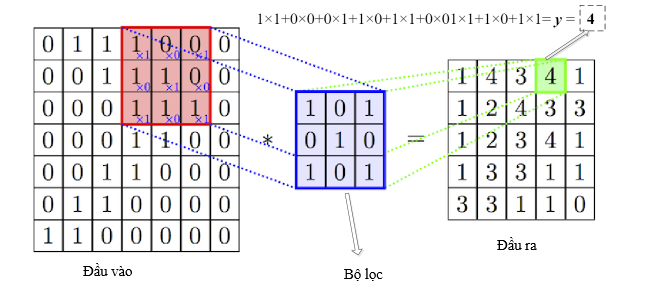
\includegraphics[width=1\textwidth]{tichchap.png}
	\caption{Ví dụ về tích chập}
	\label{fig:hinh_tichchap}
\end{figure}

{\fontsize{13}{12} \selectfont
Sự kết hợp của 1 hình ảnh với các bộ lọc khác nhau có thể thực hiện các hoạt động như phát hiện cạnh, làm mờ và làm sắc nét bằng cách áp dụng các bộ lọc.
Bộ lọc ở những lớp tích chập đầu tiên sẽ dùng để phát hiện đặc trưng đơn giản như cạnh ngang, dọc, chéo,\dots của bức ảnh. Bộ lọc ở lớp tích chập càng sâu thì phát hiện các đặc trưng càng phức tạp.
}


\subsection{Hàm kích hoạt}

{\fontsize{13}{12} \selectfont
	Phép toán tích chập chỉ là một phép toán tuyến tính nên cần bổ sung thêm yếu tố phi tuyến tính để đảm bảo CNN giải quyết được nhiều vấn đề.
	Hàm kích hoạt sẽ được đặt sau lớp tích chập.
	Hàm ReLu \cite{nair2010rectified} là hàm kích hoạt phổ biến được sử dụng cho CNN  \ref{fig:relu}. Trước khi hàm ReLU được áp dụng thì những hàm như sigmoid hay tanh mới là những hàm được sử dụng phổ biến.
	Relu được ưu chuộng vì tính đơn giản (lọc và thay thế các giá trị âm bằng 0), tăng độ thưa thớt của mạng và giảm vấn đề quá khớp \cite{caruana2000overfitting}.
	Ngoài ra ReLu cũng có tốc độ hội tụ nhanh hơn gấp 6 lần Tanh \cite{krizhevsky2012imagenet}.
}
\begin{figure}[H]
	\centering
	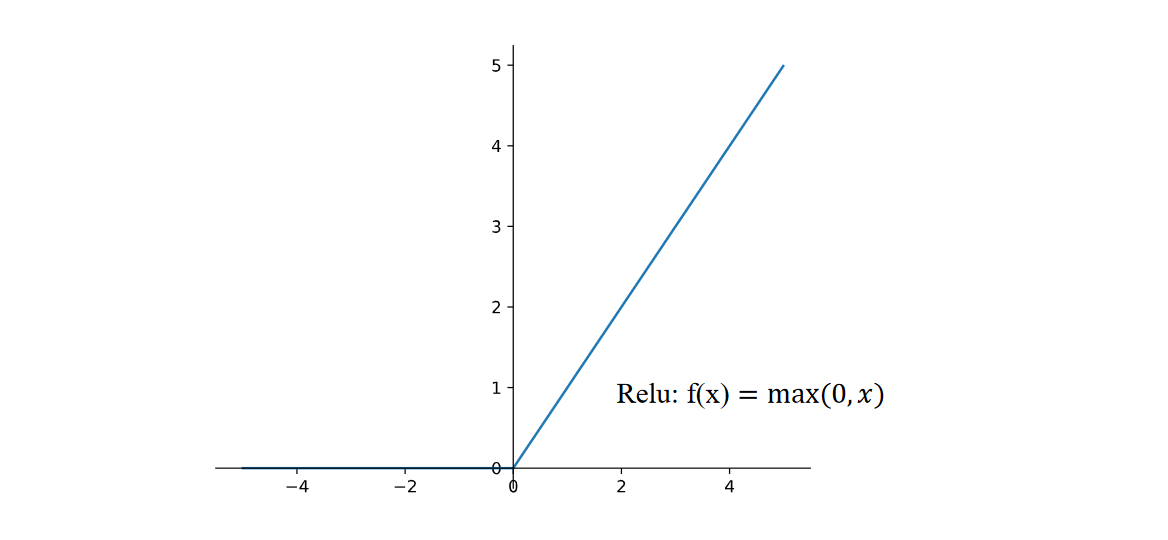
\includegraphics[width=1\textwidth]{relu.png}
	\caption{Hàm kích hoạt Relu}
	\label{fig:relu}
\end{figure}

\subsection{Lớp gộp (Polling) và Lớp kết hợp đầy đủ(Fully Connected Layer)}

{\fontsize{13}{12} \selectfont
	Lớp tích chập sẽ tạo ra nhiều đặc trưng cho ảnh đầu vào làm dữ liệu tính toán bị quá tải nếu đưa những tham số đó vào việc phân loại.
	Vì vậy lớp gộp được sử dụng trong CNN để giảm kích thước đầu vào, tăng tốc độ tính toán và hiệu năng trong việc phát hiện các đặc trưng.
	Giống như các lớp tích chập, các toán tử gộp bao gồm một cửa sổ có kích thước cố định được trượt trên tất cả các vùng đầu vào với giá trị bước trượt nhất định, tính toán một giá trị đầu ra duy nhất tại mỗi vị trí mà cửa sổ trượt qua.
	Các giá trị gộp sẽ được định sẽ thay vì có các tham số trong bộ lọc như lớp tích chập, chúng sẽ được tính bằng giá trị cực đại hoặc trung bình.
	Các phép tính này lần lượt được gọi là là gộp cực đại (max pooling) và gộp trung bình (average pooling) \ref{fig:polling}.

	Tầng cuối cùng của mô hình CNN trong bài toán phân loại ảnh là tầng kết hợp đầy đủ. Tầng này có chức năng chuyển ma trận đặc trưng ở tầng trước thành vector chứa xác suất của các đối tượng cần được dự đoán
}
\begin{figure}[H]
	\centering
	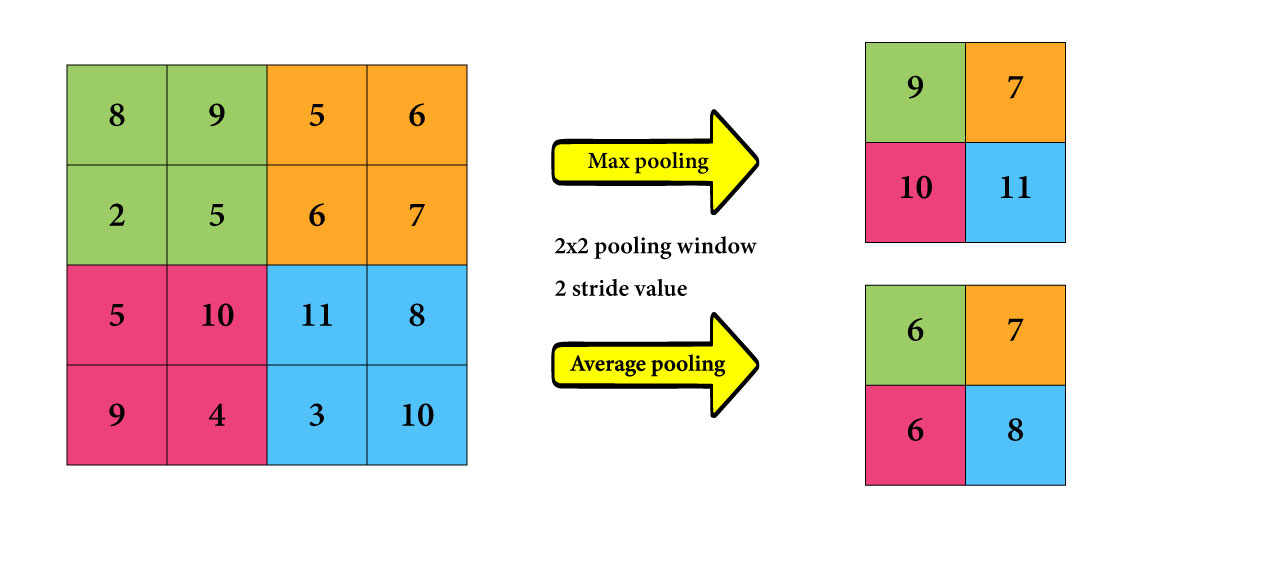
\includegraphics[width=1\textwidth]{lopgop.jpg}
	\caption{Mình họa về gộp cực đại và gộp trung bình}
	\label{fig:polling}
\end{figure}
\section{Phát hiện đối tượng}
 {\fontsize{13}{12} \selectfont
  Phát hiện đối tượng là một kĩ thuật quan trọng trong lĩnh vực Thị giác máy tính. Không chỉ nhận ra một đối tượng,
  phát hiện đối tượng sẽ vẽ các hộp giới hạn xung quanh (bbox) các đối tượng được phát hiện, từ đó
  cho phép xác định vị trí và nhãn của chúng.

  Phát hiện đối tượng được sử dụng rộng rãi trong nhiều lĩnh vực như trong công nghệ xe tự hành,
  cần lên lộ trình bằng cách xác định các vị trí của phương tiện di chuyển, người đi đường, đường xá và các vật cản trong các ảnh được thu về từ video. Hay các hệ thống an ninh cần phát hiện các mục tiêu bất thường, ví dụ như các đối tượng xâm nhập bất hợp pháp.
  Ngoài các thuật toán phát hiện đối tượng truyền thống, hiện nay các mô hình phát hiện đối tượng được phân làm 2 loại chính là mô hình phát hiện đối tượng hai giai đoạn và mô hình phát hiện đối tượng một giai đoạn.
 }
\subsection{Thuật toán Histrogram of oriented gradient (HOG)}
{\fontsize{13}{12} \selectfont
	HOG là một trong những phương pháp phát hiện đối tượng lâu đời nhất \cite{dalal2005histograms}. Nó được giới thiệu lần đàu vào năm 1986,
	tuy nhiên đến năm 2005 mới được bổ sung và sử dụng rộng rãi. HOG hoạt động trên một cửa sổ, là vùng có kích thước pixel cố định trên hình ảnh. Một cửa sổ được chia thành các vùng không gian nhỏ, được gọi là một khối và một khối còn được chia thành nhiều ô.
	Thuật toán sẽ tính toán độ lớn và hướng của độ dốc trong ô và tạo biểu đồ về hướng của độ dốc. Sau đó các biểu đồ trong cùng một khối sẽ được nối với nhau.
	Kết quả sau bước chuẩn hóa sẽ là một vector đặc trưng có tính bất biến đối với các thay đổi về điều kiện ánh sáng.

	Mục đích của HOG là trừu tượng hóa đối tượng bằng cách trích xuất ra những đặc trưng của đối tượng đó và bỏ đi những thông tin không hữu ích.
	Vì vậy, HOG đặc biệt hiệu quả trong việc phát hiện các vật thể có kết cấu và kiểu dáng có thể phân biệt được, khiến nó trở thành lựa chọn phổ biến cho các nhiệm vụ như phát hiện người đi bộ và các hình thức nhận dạng vật thể khác.
	Tuy nhiên, có nhiều chi tiết cầm phải lưu ý như HOG có nhiều tham số, bao gồm kích thước của cửa sổ, khối và ô. Điều này cũng xác định kích thước và tỷ lệ khung hình của hộp giới hạn.
	Thứ hai, HOG rất nhạy cảm với chuyển động quay. Do đó, nếu hình ảnh bị nghiêng, vector đặc trưng thu được từ HOG có thể không hữu ích cho việc phát hiện đối tượng.
	Cuối cùng, mỗi khung giới hạn sẽ tạo ra một vector HOG khác nhau, ngay cả khi tất cả chúng đều xác định cùng một đối tượng. Bạn cần một cách thông minh để biết liệu đối tượng có được phát hiện hay không, thường là mô hình học máy.
	Một số mô hình có thể được sử dụng để so sánh HOG làm vector đặc trưng để huấn luyện, điển hình như SVM.
}
\section{Các mô hình phát hiện đối tượng hai giai đoạn }
 {\fontsize{13}{12} \selectfont
  Các mô hình phát hiện đối tượng hai giai đoạn sẽ có bước đầu tiên là sử dụng mạng thiết kế khu vực để tạo ra các khu vực quan tâm có xác suất cao là đối tượng.
  Bước thứ hai là phát hiện đối tượng, thực hiện phân loại cuối cùng và định vị hộp giới hạn của các đối tượng.
  Các mô hình hai giai đoạn được dùng để giải quyết các bài toán định vị và nhận dạng đối tượng tĩnh (hình ảnh) do yêu cầu cao về độ chính xác nhưng không yêu cầu quá cao về tốc độ.
  Các mô hình tiêu biểu gồm các mô hình thuộc họ RCNN.
 }
\subsection{Mô hình R-CNN}
{\fontsize{13}{12} \selectfont
	Mô hình R-CNN được giới thiệu lần đầu vào năm 2014 \cite{girshick2014rich} cho nhiệm vụ phát hiện đối tượng và đặt những tiền đề đầu tiên cho mạng nơ-ron tích chập
	trong việc định vị, phát hiện đối tượng. Đầu tiên R-CNN sẽ trích xuất ra khoảng 2000 vùng ảnh từ ảnh đầu vào bằng cách sử dụng một giải thuật chọn lọc được gọi là selective search (tìm kiếm chọn lọc) \cite{uijlings2013selective}.
	Sau đó các vùng ảnh này sẽ được một mạng CNN tính toán và trả về kết quả các nhãn được dự đoán.
}
\begin{figure}[H]
	\centering
	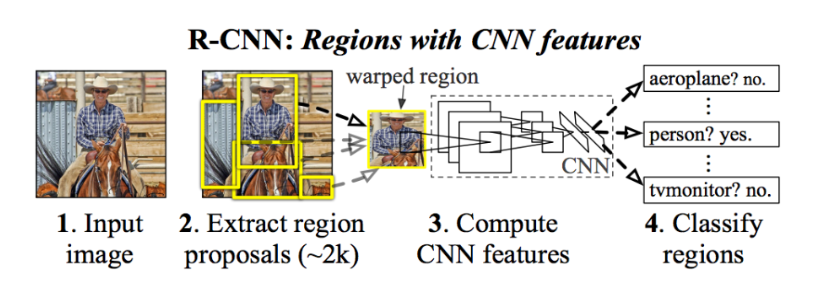
\includegraphics[width=1\textwidth]{rcnn.png}
	\caption{Mô hình CNN \cite{girshick2014rich}}
	\label{fig:rcnn}
\end{figure}
{\fontsize{13}{12} \selectfont
Hình \ref{fig:rcnn} cho thấy mô hình R-CNN cụ thể gồm những bước như sau:



{\fontsize{13}{12} \selectfont
Tuy đạt được hiệu quả ở độ chính xác khi phát hiện đối tượng và không bị ảnh hưởng bởi các đối tượng có tỉ lệ, kích thước khác nhau.
Nhưng mô hình R-CNN bị hạn chế bơi khả năng phức tạp ở tính toán, có quá nhiều thành phần độc lập làm việc tuần tự kéo làm thời gian huấn luyện mô hình chậm.
}
\begin{itemize}
	\item Thực hiện tìm kiếm chọn lọc để trích xuẩt ra các vùng đề xuất của hình ảnh dựa vào việc hợp nhất các vùng có các đặc trưng tương tự như kết cấu, màu sắc và đường viền. Mỗi vùng đề xuất này có hoặc không chứa vật thể và được bao bởi các hộp giới hạn.
	\item Chọn một CNN được đào tạo trước không gồm lớp phân loại, ở bài báo của tác giả xử dụng mô hình AlexNet. Các vùng đề xuất sẽ được thay đổi kích thước đề phù hợp vơi mạng CNN đã chọn (224x224 vơi AlexNet).
	\item Nhận được một vector đặc trưng của đối tượng khi đưa các vùng đề xuất vào mạng CNN.
	\item Vector đặc trưng trên sẽ được đào tạo qua mô hình SVM để gán nhãn.
	\item Ngoài việc phân loại đối tượng, R-CNN còn thực hiện hồi quy hộp giới hạn. Đối với mỗi lớp, một mô hình hồi quy riêng biệt được đào tạo để tinh chỉnh vị trí và kích thước của hộp giới hạn xung quanh đối tượng được phát hiện. Hồi quy hộp giới hạn giúp cải thiện độ chính xác của bằng cách điều chỉnh hộp giới hạn được đề xuất ban đầu để phù hợp hơn với ranh giới thực tế của đối tượng.
\end{itemize}
}
\bigskip
\subsection{Mô hình Fast R-CNN}
{\fontsize{13}{12} \selectfont
	Dựa vào thành công và những mặt hạn chế của R-CNN, nhóm tác giả tiếp tục phát triển mô hình Fast R-CNN vào một năm sau đó \cite{girshick2015fast}.
	Mô hình Fast R-CNN giải quyết được vấn đề huấn luyện độc lập từng thành phần giúp giải quyết được vấn đề tốc độ huấn luyện và giảm tải bộ nhớ khi không phải lưu lại vector đặc trưng cho từng lớp để huấn luyện SVM.
	Không giống như R-CNN từng vùng đề xuất được qua CNN thì ở Fast R-CNN ảnh sẽ được đưa qua CNN. Điều này giúp chia sẻ tính toán và cũng giảm thời gian huấn luyện xuống rất nhiều do nhiều vùng đề xuất chồng chập với nhau.

	Hình \ref{fig:fastrcnn} mô tả kiến trúc của Fast R-CNN, Fast R-CNN lấy đầu vào là toàn bộ hình ảnh và một tập hợp các đề xuất đối tượng. Sau đó mô hình sẽ xử lí toàn bộ hình ảnh với một số lớp tích chập kết hợp với lớp gộp tối đa để tạo ra được bản đồ đặc trưng.
	Dựa vào tìm kiếm chọn lọc, mô hình tìm được các vùng quan tâm (Region of interest pooling) hay gọi là ROI, lớp tổng hợp ROI có thể ánh xạ các ROI với sẽ trích xuất một vector đặc trưng có độ dài cố định từ các bản đồ đặc trưng. Mỗi vector đặc trưng này sẽ được đưa vào mỗi chuỗi các vector ở lớp kết nối đầy đủ \cite{girshick2015fast}.
	Fast R-CNN không sử dụng SVM làm bộ phân loại. Tầng cuối cùng sử dụng các vector được sinh ra từ lớp ROI được chia ra hai nhánh, một nhánh làm nhiệm vụ phân loại thông qua hàm softmax và một nhánh xác định tọa độ của hộp giới hạn. Hai tác vụ này sẽ tính toán song song nhau và được coi như một phần của mạng nơ-ron.
}

\begin{figure}[H]
	\centering
	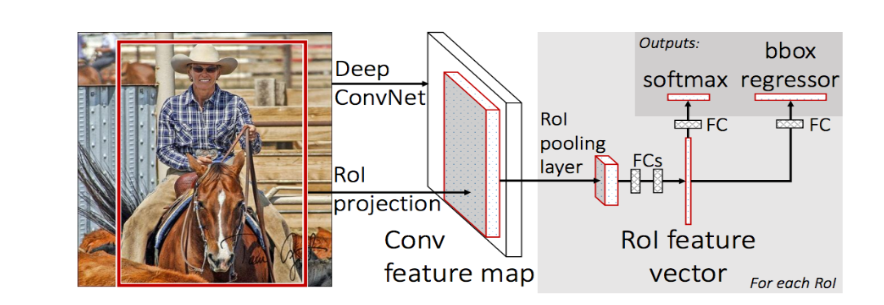
\includegraphics[width=1\textwidth]{fastrcnn.png}
	\caption{Mô hình Fast R-CNN \cite{girshick2015fast}}
	\label{fig:fastrcnn}
\end{figure}
\bigskip
{\fontsize{13}{12} \selectfont
	Tuy đã giải quyết được những vấn đề hạn chế của R-CNN như giảm thời gian rất nhiều (giảm gần 10 lần), Fast R-CNN vẫn còn sử dụng tìm kiếm chọn lọc để tạo ra các vùng đề xuất nên làm giới hạn hiệu suất của Fast R-CNN. Việc này rất dễ nhìn thấy hình \ref{fig:timefastrcnn},
	thời gian thử nghiệm lên tới 2 giây nên không đảm bảo áp dụng cho phát hiện đối tượng ở thời gian thực.
}
\begin{figure}[H]
	\centering
	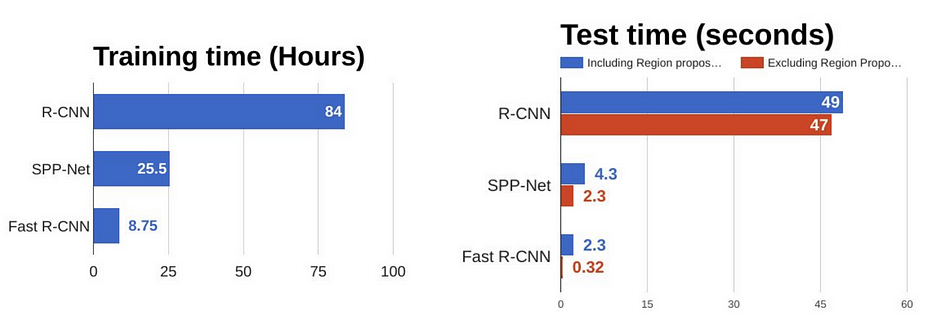
\includegraphics[width=1\textwidth]{time_fastrcnn.png}
	\caption{Thời gian huấn luyện R-CNN, SPP-NET \cite{He_2014}, Fast R-CNN \cite{testtimefastrcnn}}
	\label{fig:timefastrcnn}
\end{figure}
\bigskip



\subsection{Mô hình Fast R-CNN}
{\fontsize{13}{12} \selectfont

	Faster R-CNN là mô hình cải thiện được nhược điểm của các mô hình tiền nhiệm trong họ R-CNN. Mô hình được đề xuất bởi
	Shaoqing Ren và các cộng sự tại Microsoft Research \cite{ren2016faster} đã
	đạt kết quả tốt về tốc độ huấn luyện và phát hiện. Tương tự như Fast R-CNN, nó sử dụng mạng CNN để trích xuất feature map.
	Tuy nhiên thay vì sử dụng tìm kiếm chọn lọc để xác định các vùng đề xuất thì Faster R-CNN sử dụng mạng đề xuất vùng (RPN) để dự đoán các vùng có khả năng chứa đối tượng của ảnh.
	Sau khi thực hiện RPN, các bước xử lý sau tương tự như Fast-RCNN nhưng nhanh hơn.

	Kiến trúc của Faster R-CNN có thể được miêu tả bằng hai mạng chính như Hình \ref{fig:fasterrcnn} bao gồm mạng RPN để đề xuất các vùng và mạng Fast-RCNN.

}
\begin{figure}[H]
	\centering
	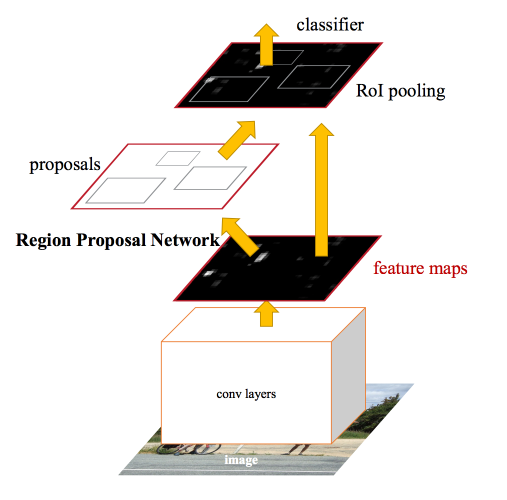
\includegraphics[width=1\textwidth]{fasterrcnn.png}
	\caption{Mô hình faster RCNN \cite{ren2016faster}}
	\label{fig:fasterrcnn}
\end{figure}
\bigskip
{\fontsize{13}{12} \selectfont
	Mạng RPN (Hình \ref{fig:rpn}) sẽ được dùng để đề xuất các vùng khả năng cao chứa đối tượng thay cho thuật toán tìm kiếm chọn lọc.
	Mạng này bao gồm các lớp tích hợp mà từ đó chúng ta có thể thu được các đặc trưng cần thiết thông qua từng lớp tích chập liên tiếp nhau.
	Để đưa ra các vùng đặc trưng, chúng ta sử dụng các hộp neo với các tỉ lệ, kích thước và độ lớn khác nhau. Đối với mỗi hộp neo tại RPN, chúng ta thực hiện phân lớp nhị phân để phân loại vùng chọn đó có khả năng chứa đối tượng hay không và dự đoán ra các hộp giới hạn đối tượng tương ứng.
	Để xác định một hộp neo có chứa đối tượng cần phải so sánh với các hộp dự đoán thật, nếu điểm của khu vực cao hơn ngưỡng trên được xem là mẫu có đối tượng, thấp hơn ngưỡng dưới là mẫu không có đối tượng, còn những điểm trong khoảng thì bỏ qua, ở bài viết ngưỡng trên và dưới lần lượt là 0.7 và 0.3.
	Các vùng đề xuất này tiếp tục đi qua lớp ROI để cố định kích thước đầu ra, sau đó phần xử lí tiếp theo tương tự như Fast-RCNN (Hình \ref{fig:fasterrcnn}).
	Với việc chia sẽ trọng số của mạng RPN và mạng Fast-RCNN. Faster R-CNN cho phép hệ thống phát hiện đối tượng đạt độ chính xác cao và chạy ở khung hình gần như thời gian thực.
}
\begin{figure}[H]
	\centering
	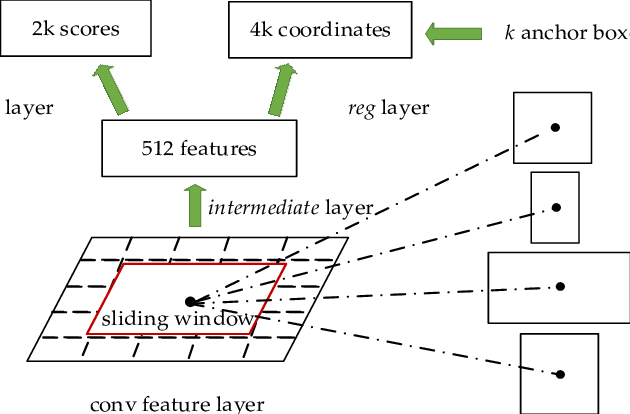
\includegraphics[width=1\textwidth]{RPN.png}
	\caption{Cấu trúc mạng RPN}
	\label{fig:rpn}
\end{figure}
\bigskip

{\fontsize{13}{12} \selectfont
	Nhìn chung các mô hình phát hiện đối tượng hai giai đoạn
	trước tiên sẽ trích xuất các vùng ứng đề xuất từ hình ảnh, sau đó tinh chỉnh kết quả phát hiện dựa trên các vùng này. Quá trình này phụ thuộc rất nhiều vào thu thập và gán nhãn hộp giới hạn cho dữ liệu.
	Mặc dù độ chính xác phát hiện cao hơn nhưng các thuật toán này lại chậm hơn so với các mô hình một giai đoạn.
	Do đó, các mô hình phát hiện hai giai đoạn chủ yếu được sử dụng trong lĩnh vực y tế, nơi độ chính xác phân loại quan trọng hơn tốc độ.
}


\section{Các mô hình phát hiện đối tượng một giai đoạn}
 {\fontsize{13}{12} \selectfont
  Các mô hình phát hiện đối tượng một giai đoạn sẽ trực tiếp từ hình ảnh đến phân loại và tọa độ hộp giới hạn.
  Các hình ảnh được đưa vào trình trích xuất đối tượng bằng CNN và sau đó các đối tượng được trích xuất sẽ được sử dụng trực tiếp để phân loại và hồi quy tọa độ hộp giới hạn.
  Phát hiện đối tượng một giai đoạn rất nhanh và có thể được sử dụng theo thời gian thực nhưng đôi khi hiệu suất lại kém phát hiện đối tượng hai giai đoạn.


  \subsection{Mô hình Yolo}}
 {\fontsize{13}{12} \selectfont
  Yolo - “You only look once” \cite{redmon2016look} là mô hình phát hiện đối tượng một giai đoạn được giới thiệu lần đầu vào năm 2015 và hiện có nhiều phiên bản cải tiến theo thời gian,
  nổi bật như Yolo, Yolov2, Yolov3, Yolov5, Yolov7 và gần nhất là Yolov8 (Hình \ref{fig:timelimeyolo}). Các mô hình Yolo không phải là thuật toán tốt nhất về độ chính xác nhưng luôn đảm bảo về tốc độ, phù hợp để xử lí các tác vụ thời gian thực.
 }
\begin{figure}[H]
	\centering
	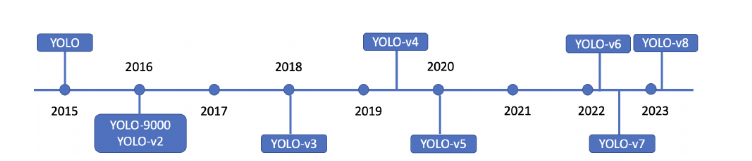
\includegraphics[width=1\textwidth]{timelineYolo.png}
	\caption{Dòng thời gian phát hiển của Yolo}
	\label{fig:timelimeyolo}
\end{figure}
\bigskip

\subsubsection{Yolo}
{\fontsize{13}{12} \selectfont
	Phương pháp chính dựa trên một mạng nơ ron duy nhất được huấn luyện dạng mô hình từ đầu cuối.
	Mô hình lấy input là một bức ảnh và dự đoán các hộp giới hạn và nhãn lớp cho mỗi hộp đó.
	Do không sử dụng các vùng đề xuất nên kỹ thuật này có độ chính xác thấp hơn do có thể bị nhiều lỗi định vị vật thể,
	Yolo có thể hoạt động ở tốc độ 45 khung hình/giây (fps) và tối đa 155 fps cho phiên bản tối ưu hóa tốc độ. Tốc độ này còn nhanh hơn cả tốc độ khung hình của máy quay phim thông thường chỉ vào khoảng 24 fps.

}

\begin{figure}[H]
	\centering
	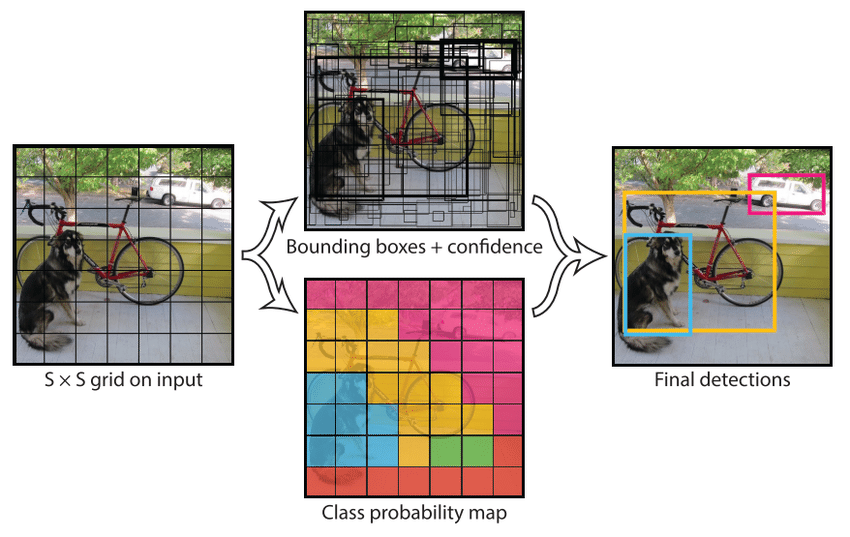
\includegraphics[width=1\textwidth]{yolo.png}
	\caption{Mô hình hệ thống Yolo}
	\label{fig:yolo}
\end{figure}
\bigskip


{\fontsize{13}{12} \selectfont
	Hình \ref{fig:yolo} mô tả hoạt động của mô hình Yolo bằng cách phân chia hình ảnh đầu vào thành một lưới gồm các ô có kích thước
	$S \times S$. Nếu tâm của đối tượng cần xác định rơi vào một ô nào đó thì ô đó sẽ có nhiệm nhiệm xác định đối tượng đó và hộp giới hạn của nó.
	Mỗi ô lưới dự đoán các hộp giới hạn và điểm tin cậy về khả năng chứa vật thể của các hộp đó, độ tin cây được tính bằng $Pr(Object) * IOU^{pred}_{truth}$ \cite{redmon2016look}
	với $Pr(Object)$ là xác suất có một đối tượng được chứa bên trong hộp giới hạn, $IOU^{pred}_{truth}$ tỉ lệ của hộp giới hạn được dự đoán so với hộp giới hạn thật của đối tượng.
	Nếu không có đối tượng tồn tại trong ô, độ tin cây sẽ bằng 0. Mỗi hộp giới hạn trong Yolo được biểu diễn bằng năm tham số
	$x$, $y$, $w$, $h$, và độ tin cậy. Trong đó ($x$, $y$) là tọa độ tâm, $w$ là chiều rộng và $h$ là chiều cao của hộp giới hạn.
	Kết quả của mạng sẽ thu được một ma trận khối 3 chiều (tensor)  $S \times S \times (B * 5 + C)$ giá trị, với
	$C$ là số lượng lớp của bài toán. Ví dụ như tác giả có đề cập việc đánh giá trên tập dự liệu PASCAL VOC, $S = 7, B = 2, C = 20$, kết quả đầu ra sẽ là $7 \times 7 \times 30$.
	Hình \ref{fig:mangyolo} mô tả kiến trúc của Yolo gồm 24 lớp chập theo sau là 2 lớp được kết nối đầy đủ. Các lớp chập $1 \times 1$ xen kẽ làm giảm không gian đặc trưng của các lớp trước đó.
	Có thể dễ dàng nhận thấy rằng toàn bộ mạng Yolo à không có bất kỳ cấu trúc mạng con nào nên Yolo sẽ nhanh hơn các mô hình phát hiện hai giai đoạn.
}

\begin{figure}[H]
	\centering
	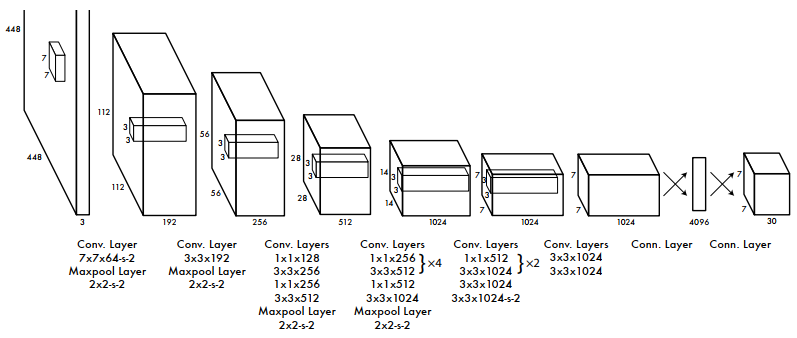
\includegraphics[width=1\textwidth]{yolo_a.png}
	\caption{Kiến trúc mạng Yolo}
	\label{fig:mangyolo}
\end{figure}
\bigskip

\subsubsection{Yolov2}
{\fontsize{13}{12} \selectfont

	Yolov2 \cite{redmon2016yolo9000}, còn được gọi là Yolo9000, được giới thiệu vào năm 2016 như một cải tiến so với thuật toán Yolo ban đầu. Nó được thiết kế để nhanh hơn, chính xác hơn Yolo và có thể phát hiện nhiều loại đối tượng hơn.
	Yolov2 giải quyết một số vấn đề ở Yolo ban đầu tăng tỉ lệ dự đoán được ví trí vật thể, phát hiện được các vật thể gần nhau.
	Ở 67 FPS, YOLOv2 đạt được 76.8\% mAP trên VOC 2007. Ở 40 FPS, YOLOv2 đạt 78.6\% mAP.
	Đầu tiên Yolov2 sẽ thực hiện chuẩn hóa hàng loạt (batch normalization) giúp cải thiện độ ổn định, giảm hiện tượng quá khớp. So với Yolo sử dụng hình ảnh $224 \times 224$ để huấn luyện và $448 \times 448$
	để phát hiện (detect)  làm cho mạng phải chuyển độ phân giải trong lúc huấn luyện, làm giảm chất lượng hình ảnh, Yolov2 sẽ thực hiện fine-tuning một mạng phân lớp với 10 epochs trên tập ImageNet.
	Điều này giúp mạng có thời gian điều chỉnh các bộ lọc để hoạt động tốt hơn trên ảnh đầu vào có độ phân giải cao.

	Tiếp theo, Yolov2 loại bỏ tầng kết nối đầy đủ để thay thế bằng việc sử dụng ý tưởng hộp neo của FasterRCNN,
	điều này giúp việc xác định các hộp giới hạn chính xác hơn và loại bỏ được ràng buộc mỗi ô chỉ được dự đoán một đối tượng như Yolo.
	Tuy nhiên khi sử dụng hộp neo thì kích thước được tạo ngẫu nhiên, mặc dù mạng có thể học để tạo hộp neo một cách hợp lý nhưng một hộp neo được tạo
	ban đầu đủ tốt sẽ giúp việc mạng được cải thiện tốt hơn. Yolo2 sẽ sử dụng k-mean dựa trên các hộp giới hạn để tìm kích thước hộp neo phù hợp nhất cho mạng.
	Yolov2 cũng sử dụng vị trí tương
	đối của neo và ô lưới để làm cho neo không bị lệch khỏi tâm của đối tượng. Điều này
	làm cho mạng ổn định hơn và dễ hội tụ hơn. Hơn thế nữa, Yolov2 có kích thước bản đồ đặc trưng là $13 \times 13$ đủ để phát hiện các đối tượng có kích thước lớn và khắc phục nhược điểm của Yolo là khó khắn trong việc nhận dạng các vật thể nhỏ
	bằng cách đưa vào các lớp chuyển tiếp để nối các bản đồ đặc trưng của lớp trước đó với các bản đồ đặc trưng của các lớp sau ở kích thước $26
		times 26$. Điều đặc biệt của Yolov2 mang lại là một kiến trúc mạng mới được gọi là Darknet-19.
	Mạng bao gồm 19 lớp tích chập và 5 lớp gộp lấy giá trị lớn nhất, đồng thời loại bỏ tầng kết nối đầy đủ, việc này làm tăng đáng kể tốc độ của mạng.
	Hình \ref{fig:yolov2} dưới đây mô tả kiến trúc cụ thể của Darknet-19.

}

\begin{figure}[H]
	\centering
	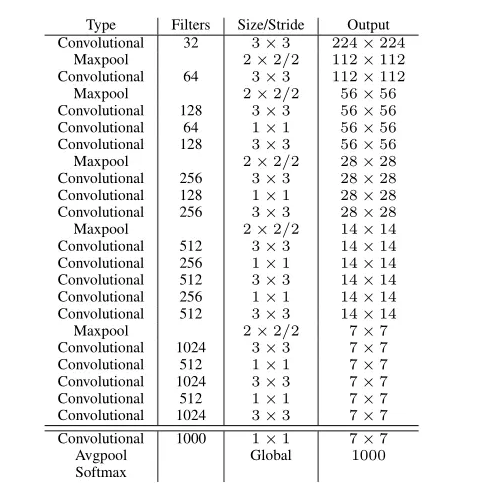
\includegraphics[width=1\textwidth]{yolov2.png}
	\caption{Kiến trúc mạng Darknet-19 \cite{deterseong}}
	\label{fig:yolov2}
\end{figure}
\bigskip

\subsubsection{Yolov3}
{\fontsize{13}{12} \selectfont
	Năm 2018, Yolov3 \cite{redmon2018yolov3} đưa ra những sự điều chỉnh nhỏ so với phiên bản trước đó, đầu tiên Yolov3 hàm softmax để phân loại mà thay vào đó sử dụng
	hàm logistic giúp tăng khả năng nhận dạng các vật thể khi ở gần nhau. Một cải tiến khác trong Yolov3 là các hộp neo với các tỉ lệ và khung hình khác nhau. Trong Yolo2 các hộp neo này đều có cùng kích thước
	nên làm giảm khả năng phát hiện các đối tượng có kích thước và hình dạng khác nhau của thuật toán. Yolov3 dự đoán các hộp giới hạn tại ba cấp độ phóng đại (scale) khác nhau của bản đồ đặc trưng sử dụng cơ chế mạng kim tự tháp (FPN)  \cite{lin2017feature}
	giúp trích xuất các đặc điểm đối tượng bị chồng chéo chính xác hơn. Cuối cùng, Yolov3 sử dụng mạng Darknet-53 với bao gồm 53 lớp tích chập, cải thiện đáng kẽ so với Darknet-19 của Yolov2.
	Yolov3 sử dụng các lớp tích chập có kích thước $3 \times 3 $ và $1 \times 1$ kế tiếp nhau, mô hình mạng Darket-53 như \ref{fig:yolov3}. So với Yolov2 thì Yolov3 đã cải thiện độ chính xác, nhất là ở những vật thể nhỏ, tuy nhiên thời gian huấn luyện sẽ lâu hơn vì cấu trúc mạng sâu hơn.

}

\begin{figure}[H]
	\centering
	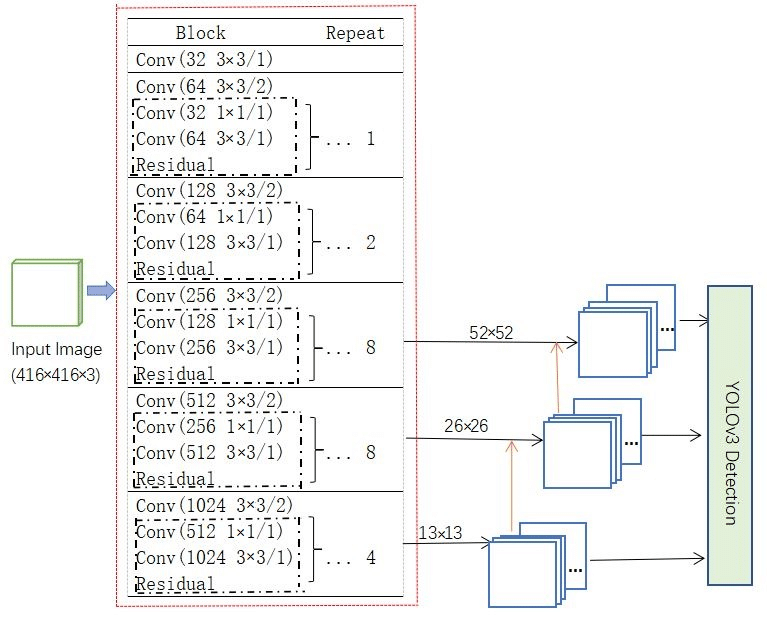
\includegraphics[width=1\textwidth]{yolov3.png}
	\caption{Kiến trúc mạng Darknet-53 \cite{detectiongao2021}}
	\label{fig:yolov3}
\end{figure}
\bigskip
\subsubsection{Yolov4}
{\fontsize{13}{12} \selectfont
	Yolov4 là phiên bản thứ tư của thuật toán phát hiện đối tượng họ Yolo được giới thiệu vào năm 2020 \cite{bochkovskiy2020yolov4} như một cải tiến so với Yolov3 bằng cách áp dụng các phương pháp hiện đại.
	Trong đó có kỹ thuật Bag of Freebies (BoF) là các kỹ thuật giúp cải thiện độ chính xác của mô hình trong quá trình đào tạo mà không làm tăng chi phí tính toán.
	Tăng cường dữ liệu là một kỹ thuật BoF phổ biến được sử dụng trong phát hiện đối tượng, giúp tăng tính biến đổi của hình ảnh đầu vào để cải thiện độ tin cậy của mô hình. Một số ví dụ về tăng cường dữ liệu bao gồm biến dạng trắc quang (điều chỉnh độ sáng, độ tương phản, màu sắc, độ bão hòa và nhiễu của hình ảnh) và biến dạng hình học (thêm tỷ lệ ngẫu nhiên, cắt xén, lật và xoay). Những kỹ thuật này giúp mô hình khái quát hóa tốt hơn cho các loại hình ảnh khác nhau.
	Yolov4 đã giới hiệu một kiến trúc tổng thể cho các mô hình phát hiện đối tượng bao gồm các thành phần xương sống (neck), cổ (neck), đầu (head) và các lớp liên kết để tối ưu việc phát hiện đối tượng ở thời gian thực. Phần backbone được đào tạo trước trên tập ImageNet và được sử dụng để dự đoán các lớp và hộp giới hạn của đối tượng đó.
	Backbone có thể là các mô hình như VGG \cite{simonyan2015deep}, ResNet \cite{he2015deep}, RestNeXt \cite{xie2017aggregated} hoặc DensenNet \cite{huang2018densely}.
	Phần neck được sử dụng để thu thập các bản đồ đặc trưng từ các giai đoạn khác nhau và thường bao gồm các luồng đi từ dưới lên và các luồng đi từ trên xuống, từ đó giúp cho lớp nhận dạng sẽ chứa thhông tin phong phú hơn. Phần head là phần được sử dụng để thực hiện việc phát hiện và phân loại đối tượng cuối cùng.
	Kiến trúc tổng quan được Yolov4 định nghĩa như hình \ref{fig:yolov4_1}.
}
\begin{figure}[H]
	\centering
	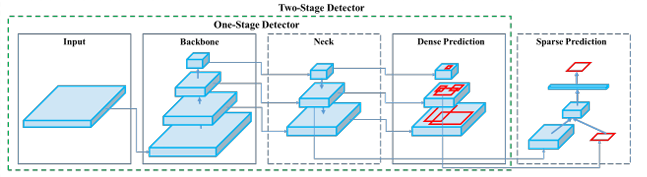
\includegraphics[width=1\textwidth]{yolov4_kt.png}
	\caption{Kiến trúc tổng quan mô hình phát hiện đối tượng \cite{bochkovskiy2020yolov4}}
	\label{fig:yolov4_1}
\end{figure}
\bigskip

{\fontsize{13}{12} \selectfont
	Yolov4 sử dụng kiến trúc CNN mới có tên là Cross Stage Partial Network (CSPNet) \cite{wang2019cspnet} và là một biến thể của kiến trúc ResNet được thiết kế đặc biệt cho các nhiệm vụ phát hiện đối tượng. Nó có cấu trúc tương đối nông, chỉ có 54 lớp chập. Tuy nhiên, nó có thể đạt được kết quả tiên tiến trên các tiêu chuẩn phát hiện đối tượng khác nhau.
	Backbone của Yolov4 sửa Darknet53 ở Yolov3 bằng cách thay thế các khối Residual Block thành CSPResBlock, tạo nên mạng CSPDarknet23.
	Yolov4 có neck là sự kết hợp ba phương pháp hiện đại khác nhau: Path Aggregation Network (PANet) \cite{liu2018path}, một khối SPP \cite{He_2014} và ba khối SAM \cite{woo2018cbam}.
	YOLOv4 có kiến trúc phần đầu giống như trong Yolov3, kiến trúc mô hình Yolov4 như hình \ref{fig:yolov4_2}.
	Thiết kế này cho phép Yolov4 thực hiện phát hiện đối tượng với tốc độ ấn tượng, phù hợp với các ứng dụng thời gian thực. Yolov4 cũng vượt trội về độ chính xác, đạt được kết quả tiên tiến trong các tiêu chuẩn phát hiện đối tượng.
	YOLOv4 là mô hình phát hiện đối tượng mạnh mẽ và hiệu quả, tạo ra sự cân bằng giữa tốc độ và độ chính xác. Việc sử dụng các tính năng độc đáo và nhiều kỹ thuật BoF trong quá trình đào tạo cho phép mô hình thực hiện xuất sắc các nhiệm vụ phát hiện đối tượng theo thời gian thực.
}
{\fontsize{13}{12} \selectfont
	\begin{figure}[H]
		\centering
		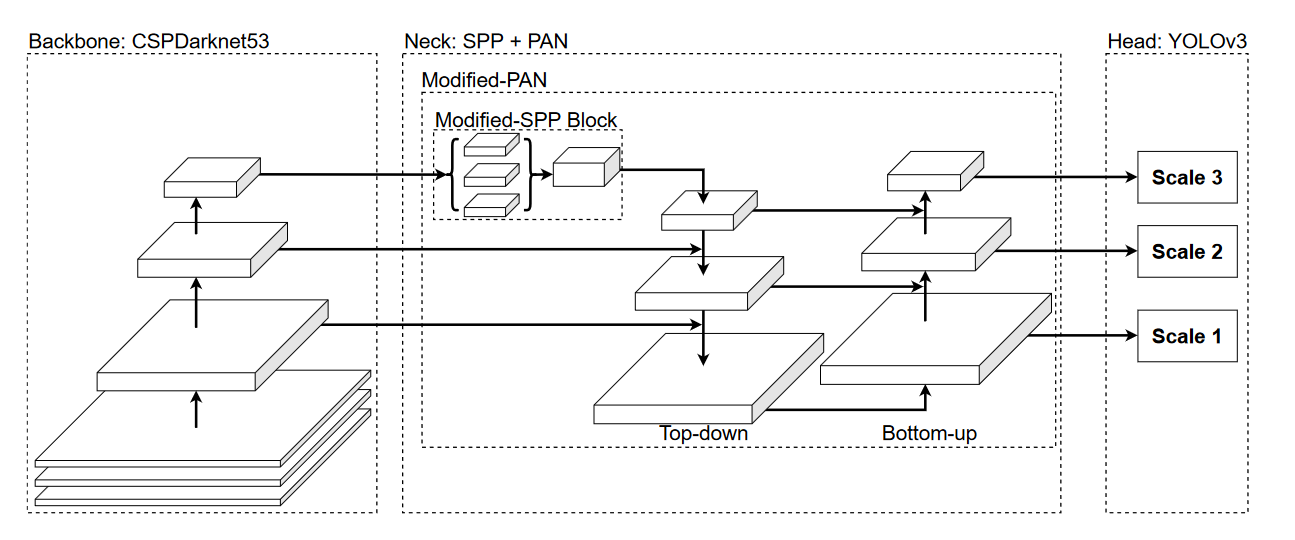
\includegraphics[width=1\textwidth]{yolov4_2.png}
		\caption{Kiến trúc Yolov4}
		\label{fig:yolov4_2}
	\end{figure}
	\bigskip

}
\subsubsection{Yolov5 và Yolov6}
{\fontsize{13}{12} \selectfont
	Yolov5 được giới thiệu vào năm 2020 bởi cùng một nhóm đã phát triển thuật toán YOLO ban đầu dưới dạng một dự án mã nguồn mở và được duy trì bởi Ultralytics.
	Thời gian phát hành của Yolov5 chỉ sau một tháng so với Yolov4, tuy nhiên thời gian nghiên cứu tương đối gần nhau. \
	Cả hai nhà nghiên cứu về cơ bản đều sử dụng những tiến bộ tiên tiến nhất trong lĩnh vực thị giác máy tính vào thời điểm đó. Do đó kiến trúc của Yolov4 và Yolov5 cực kỳ giống nhau.
	Tuy nhiên, Yolov5 sử dụng khung là Pytorch thay vì Darknet, điều này sẽ giúp cho việc cài đặt, sử dụng và phát triển dễ dàng hơn vì cộng đồng Pytorch rất đông đảo.
	Hình \ref{fig:yolov5} mô tả kiến trúc của Yolov5 không khác biệt nhiều so với Yolov4, với backbone thay thế CSPNet với ít hơn một lớp tích chập (53 lớp) gọi là C3 module, phần neck cải tiến SPP bằng SPP-Fast có khả năng xử lí nhanh hơn,
	phần head vẫn giữ là Yolov3.
}

{\fontsize{13}{12} \selectfont
	\begin{figure}[H]
		\centering
		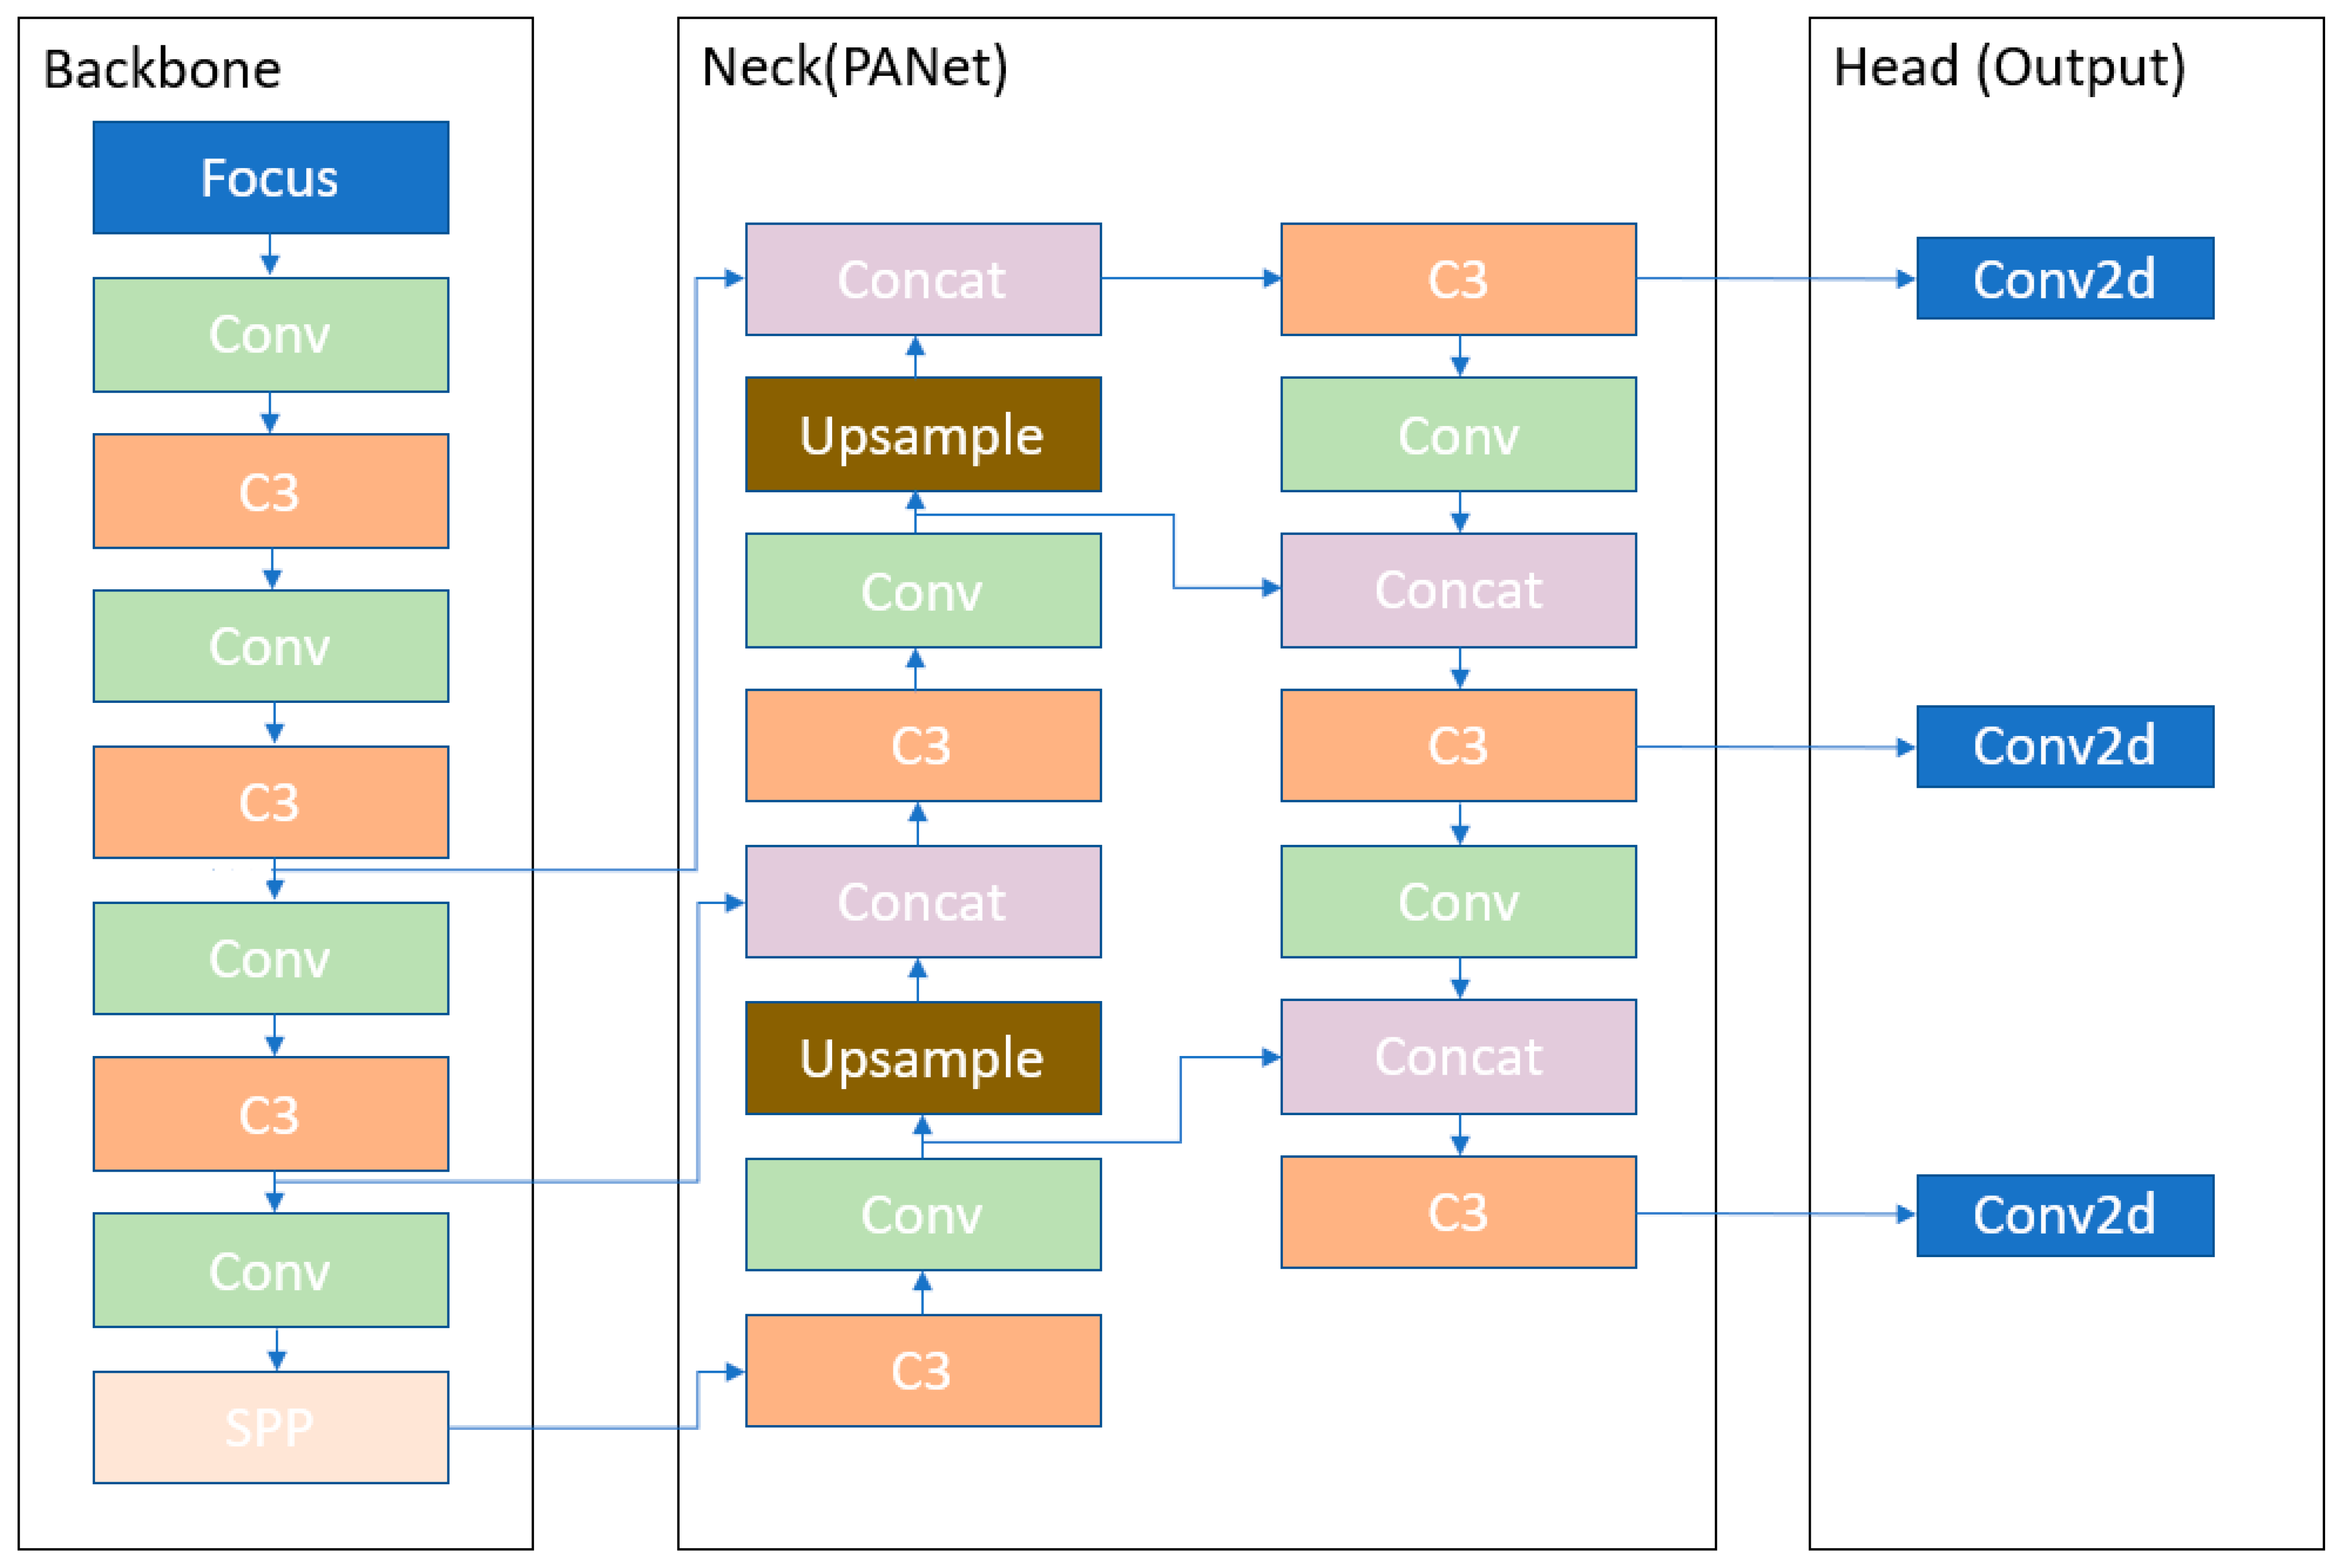
\includegraphics[width=1\textwidth]{yolov5.png}
		\caption{Kiến trúc Yolov5 \cite{s22020464}}
		\label{fig:yolov5}
	\end{figure}
	\bigskip

	YOLO v5 sử dụng một phương pháp mới để tạo các hộp neo, được gọi là hộp neo tự động.
	Nó liên quan đến việc sử dụng thuật toán phân cụm để nhóm các hộp giới hạn thực tế thành các cụm và sau đó sử dụng trọng tâm của các cụm làm hộp neo.
	Điều này cho phép các hộp néo được căn chỉnh chặt chẽ hơn với kích thước và hình dạng của các đối tượng.

	Yolov6 \cite{li2022yolov6} được đề xuất vào năm 2022 bởi Li và cộng sự như một cải tiến so với các phiên bản trước.
	Một trong những điểm khác biệt chính giữa Yolov5 và Yolov6 là kiến trúc CNN được sử dụng.
	Yolov6 sử dụng một biến thể của kiến trúc EfficientNet có tên là EfficientNet-L2 \cite{yolov72023}.
	Đó là một kiến trúc hiệu quả hơn so với EfficientDet được sử dụng trong Yolov5 với ít tham số hơn và hiệu quả tính toán cao hơn. Nó có thể đạt được kết quả tiên tiến trên các điểm chuẩn phát hiện đối tượng khác nhau.
}
\subsubsection{Yolov7}
\label{sec:yolov7}
{\fontsize{13}{12} \selectfont
	Năm 2022, Yolov7 \cite{wang2022yolov7} được công bố với những cải tiến mang lại hiệu quả cao trong các mô hình phát hiện đối tượng. Một trong những cải tiến là việc sử dụng hộp neo.
	Yolov7 sử dụng chín hộp neo, cho phép phát hiện phạm vi hình dạng và kích thước đối tượng rộng hơn so với các phiên bản trước, do đó giúp giảm số lượng xác định sai.
	Yolov7 cũng có độ phân giải cao hơn so với các phiên bản trước. Nó xử lý hình ảnh ở độ phân giải 608 x 608, cao hơn độ phân giải 416 x 416 được sử dụng trong Yolov3. Độ phân giải cao hơn này cho phép Yolov7 phát hiện các đối tượng nhỏ hơn và có độ chính xác tổng thể cao hơn.

	Một cải tiến quan trọng trong Yolov7 là việc sử dụng một hàm mất mát mới gọi là “focal loss”. Các phiên bản trước của Yolo đã sử dụng cross-entropy là một hàm mất mát tiêu chuẩn, được biết là kém hiệu quả hơn trong việc phát hiện các đối tượng nhỏ. Focal loss giải quyết vấn đề này bằng cách giảm trọng số mất mát cho các ví dụ được phân loại tốt và tập trung vào các ví dụ các đối tượng khó phát hiện.
	Một trong những ưu điểm chính của Yolov7 là tốc độ. Nó có thể xử lý hình ảnh với tốc độ 155 khung hình mỗi giây, nhanh hơn nhiều so với các thuật toán phát hiện đối tượng hiện đại khác. Điều này làm cho nó phù hợp với các ứng dụng thời gian thực nhạy cảm như giám sát và ô tô tự lái, trong đó tốc độ xử lý cao hơn là rất quan trọng.
	So sánh hiệu suất và tốc độ của Yolov7 với các mô hình phát hiện đối tượng thời gian thực hiện đại (Hình \ref{fig:yolov7}).
}
{\fontsize{13}{12} \selectfont
	Yolov7 tuy là thuật toán phát hiện đối tượng tương đối mạnh mẽ nhưng vẫn còn những hạn chế của các mô hình phát hiện đối tượng như gặp không đảm bảo trong việc phát hiện các đối tượng nhỏ. Mô hình có thể không phát hiện chính xác các đối tượng trong các cảnh đông đúc hoặc khi các đối tượng ở xa máy ảnh.
	Ngoài ra, Yolov7 còn gặp khó khăn khi phát hiện đối tượng rất lớn hay rất nhỏ so với các đối tượng khác trong ngữ cảnh. Cuối cùng, Yolov7 đòi hỏi nhiều tính toán, điều này gây khó khăn khi chạy trong thời gian thực trên các thiết bị hạn chế về tài nguyên như điện thoại thông minh hoặc các thiết bị
	khác.
}

\begin{figure}[H]
	\centering
	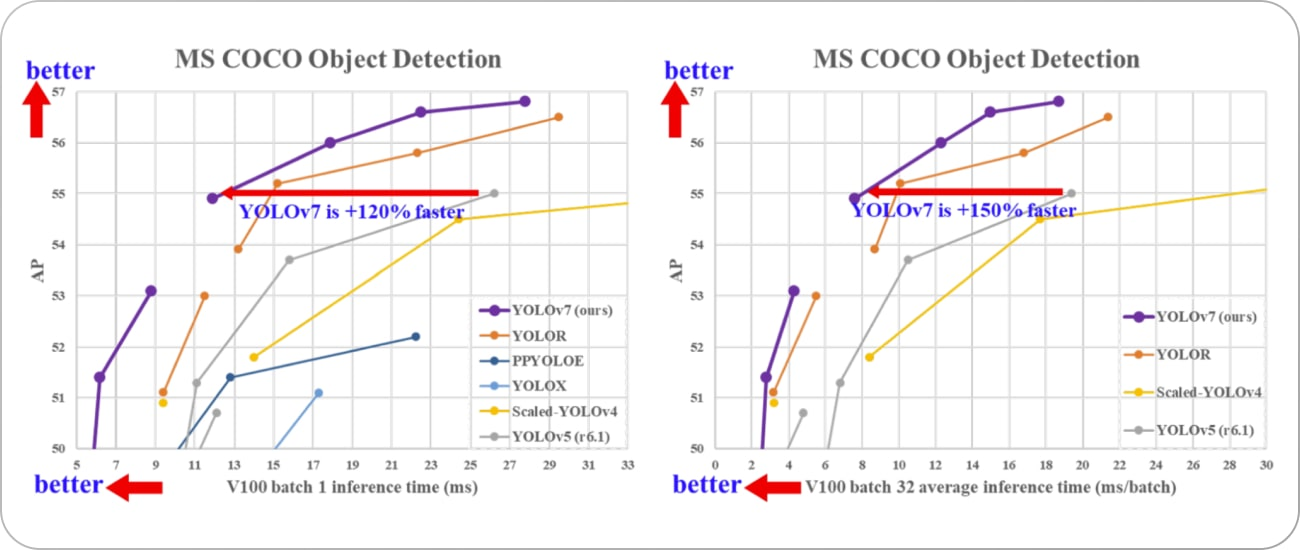
\includegraphics[width=1\textwidth]{yolov7.jpg}
	\caption{So sánh hiệu suất và tốc độ của Yolov7 \cite{wang2022yolov7}}
	\label{fig:yolov7}
\end{figure}
\bigskip

\subsubsection{Yolov8}
\label{sec:yolov8}
{\fontsize{13}{12} \selectfont
	Được công bố vào đầu năm 2023, Yolov8 đã mang lại nhiều điểm tích cực so với phiên bản tiền nhiệm, như phát hiện không dùng anchor, giới thiệu lớp tích chập C2f và tăng cường mosaic.
	Yolov8 tương tự như Yolov5 được xây dựng và duy trì bởi nhóm Ultralytics, hiện Yolov8 vẫn chưa có bài báo chính thức, tuy nhiên vẫn có thể tìm kiếm thông tin nhờ vào tài liệu và cộng đồng sử dụng Yolov8.
	YOLOv8 là mô hình không có neo. Điều này có nghĩa là nó dự đoán trực tiếp tâm của đối tượng thay vì xác định hộp neo như những mô hình trước đó.
	Điều này giúp Yolov8 linh hoạt hơn trong việc phát hiện các vật thể có hình dạng và kích thước khác nhau, đặc biệt là các vật thể mỏng hoặc nhỏ có thể không vừa với các hộp neo được xác định trước của hệ thống.
	Một lợi ích nữa của phương pháp không có neo là tính đơn giản của nó. Bằng cách loại bỏ sự phụ thuộc vào các hộp neo, mô hình trở nên dễ hiểu và dễ thực hiện hơn.
	Yolov8 còn giới thiệu một kĩ thuật mới là tăng cường dữ liệu mosiac (Hình \ref{fig:mosaic}). Tăng cường dữ liệu mosaic là một kỹ thuật đơn giản, trong đó bốn hình ảnh khác nhau được nối lại với nhau và đưa vào mô hình như đầu vào. Điều này giúp mô hình học được các đối tượng thực sự từ các vị trí khác nhau và trong trạng thái bị che khuất.
	Việc thực hiện tăng cường dữ liệu mosiac có thể làm giảm hiệu suất, vì vậy nó đã sẽ được tắt đi khi quá trình huấn luyện chuyển sang những epoch cuối cùng.
}
\begin{figure}[H]
	\centering
	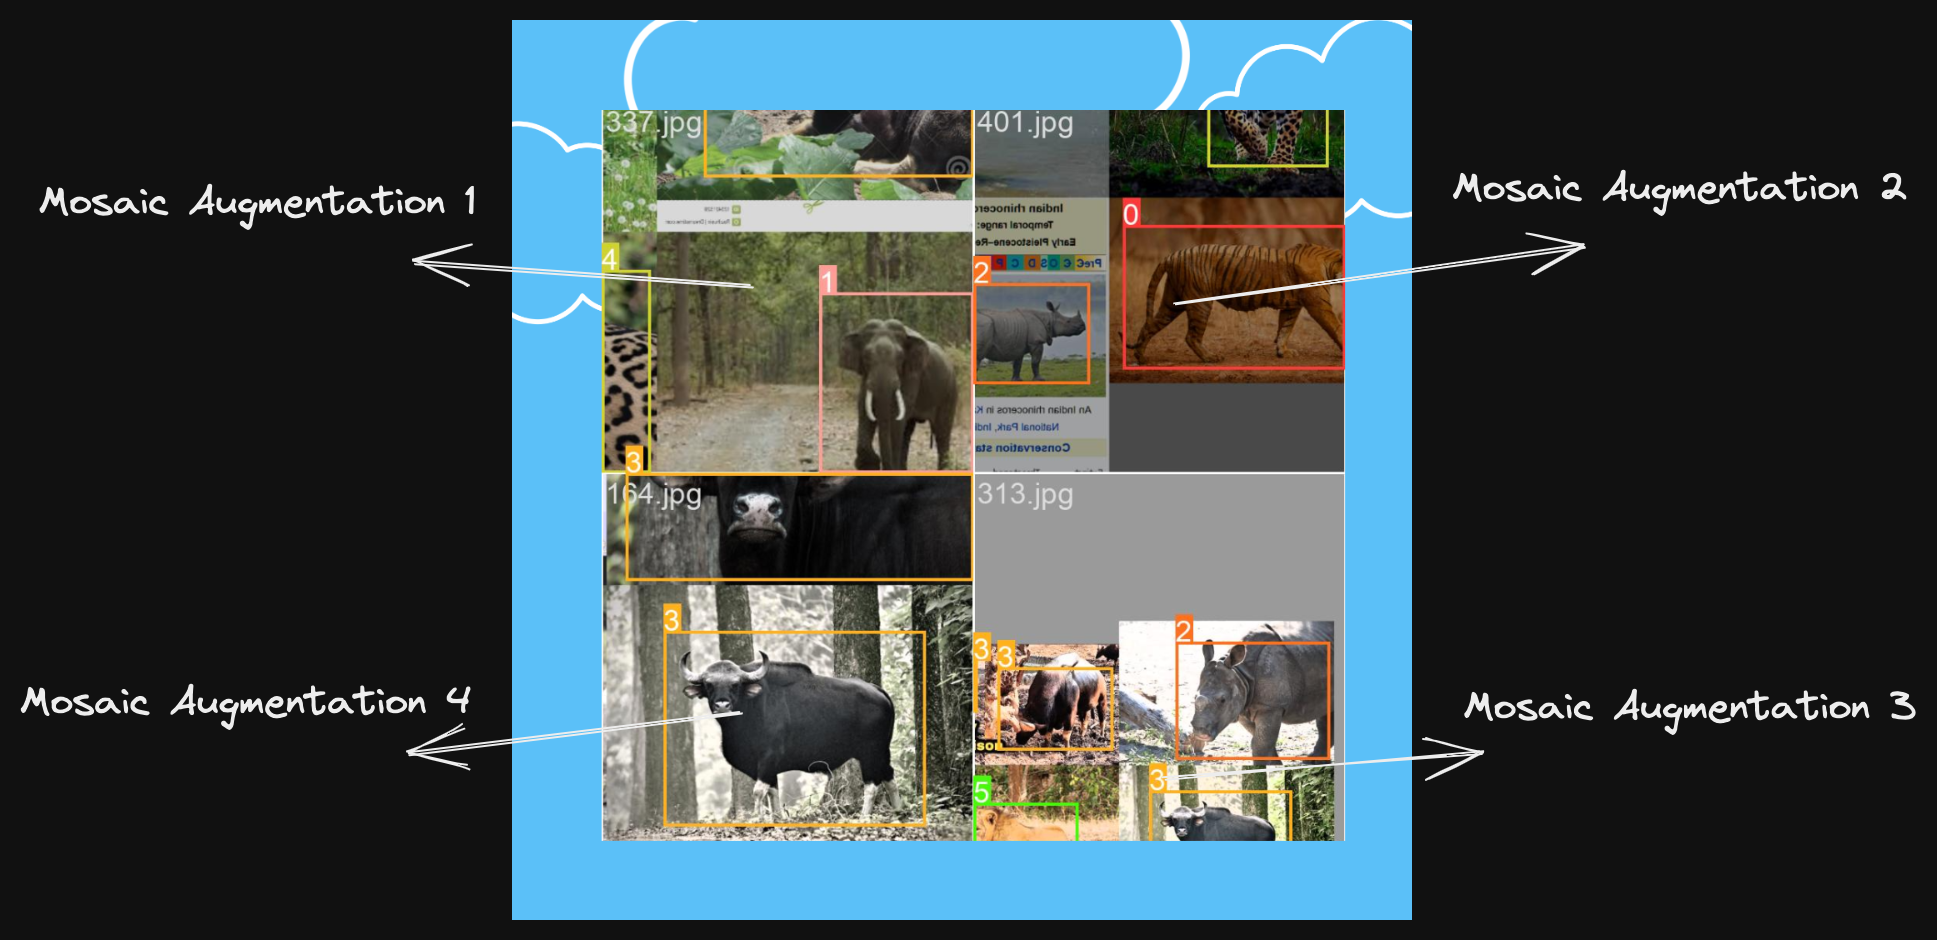
\includegraphics[width=1\textwidth]{mosiac.png}
	\caption[]{Tăng cường dữ liệu mosiac\footnotemark}
	\label{fig:mosaic}
\end{figure}
\bigskip
\footnotetext{\url{http://wandb.ai/}}
\subsection{Mô hình SSD}
{\fontsize{13}{12} \selectfont
	Tương tự như các mô hình họ Yolo, mô hình SSD \cite{Liu_2016} (Single Shot MultiBox Detector) là thuật toán phát hiện đối tượng một giao đoạn nên tỏ ra nhanh hơn so với các mô hình họ R-CNN.
	Mô hình SSD là sự kết hợp của trích xuất các bản đồ đặc trưng từ mạng CNN và áp dụng bộ lọc để phát hiện vật thể ở các độ phân giải khác nhau. SSD nhận đầu vào là các tọa độ hộp giới hạn của vật thể và nhãn của vật thể chứa trong các hộp giới hạn đó.
	Mô hình sẽ tạo ra các lưới ô trên các bản đồ đặc trưng, từ tâm của mỗi ô sẽ xác định tập hợp các hộp giới hạn mặc định được lựa chọn thủ công để dự đoán khung hình có khả năng bao quanh vật thể (Hình \ref{fig:ssd}).
	Tại mỗi hộp giới hạn mặc định, ta cần dự báo phân phối xác suất $c = (c_1, c_2,\dots, c_n)$ tương ứng với các lớp $C= C_1, C_2,\dots,C_n $ . Tại thời điểm huấn luyện, ta cần so khớp các hộp giới hạn mặc định với các hộp giới hạn thực của vật thể trên ảnh đầu vào sao cho mức độ sai số qua mất mát vị trí là thấp nhất, sau đó dự đoán nhãn bằng hàm sofmax để dự đoán nhãn.
}
\begin{figure}[H]
	\centering
	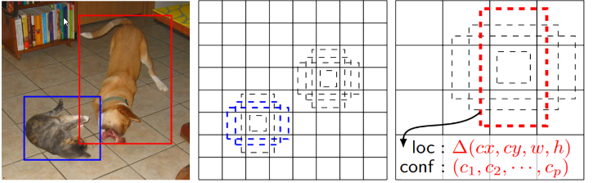
\includegraphics[width=1\textwidth]{ssd.png}
	\caption{Ví dụ về các hộp mặc định thủ công từ bản đồ đặc trưng ở SSD \cite{Liu_2016}}
	\label{fig:ssd}
\end{figure}
\bigskip

{\fontsize{13}{12} \selectfont
	Bằng việc tính toán các hộp giới hạn trên các bản đồ đặc trưng khác nhau, tại mỗi tầng chứa bản đồ đặc trưng, mỗi hộp giới hạn sẽ xác định được một phần hình ảnh với kích thước khác nhau. Như trên Hình, con mèo và con chó có thể được phát hiện ở hai tầng khác nhau với kích thước thước lần lượt là 8x8 và 4x4. Thay vì sử dụng một hộp giới hạn và thay đổi kích thước để phù hợp với vật thể thì SSD sử dụng nhiều box trên nhiều tầng, từ đó tổng hợp ra vị trí và kích thước của hộp cần xác định. Với việc loại bỏ đi vùng đề xuất khu vực, SSD sẽ đạt tốc độ xử lí cao hơn các Faster-RCNN.
	SSD sử dụng mô mạng CNN duy nhất, kiến trúc gồm hai phần với một mạng cơ sở có thể là VGG16, ResNet hay Mobinet được loại bỏ tầng kết nối đầy đủ có nhiệm vụ trích xuất ra các bản đồ đặc trưng.
	Một tập hợp các tầng tích chập phụ trợ để thay thế cho tầng kết nối bị loại bỏ. Các lớp này giảm dần kích thước không gian trong khi tăng số lượng kênh (kênh đặc trưng). hiết kế này cho phép SSD tạo ra các bản đồ đặc trưng ở nhiều tỷ lệ. Bản đồ đặc trưng của mỗi thang đo phù hợp để phát hiện các vật thể có kích thước khác nhau.
	Sau đó SSD liên kết các hộp neo mặc định được xác định trước với các bản đồ đặc trưng như đã đề cập ở trên.
	Kiến trúc được thể hiện ở hình \ref{fig:ssd2}
}

\begin{figure}[H]
	\centering
	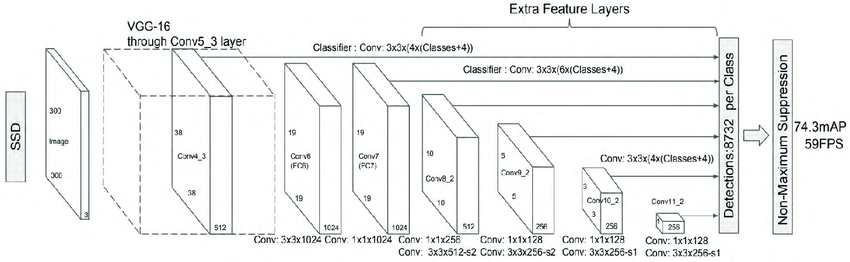
\includegraphics[width=1\textwidth]{ssd_2.png}
	\caption{Kiến trúc mô hình SSD \cite{Liu_2016}}
	\label{fig:ssd2}
\end{figure}
\bigskip

{\fontsize{13}{12} \selectfont
	SSD nổi bật nhờ hiệu suất thời gian thực, sự đơn giản và sự cân bằng tốt giữa độ chính xác và tốc độ. Nó rất phù hợp cho nhiều ứng dụng, đặc biệt là những ứng dụng yêu cầu phát hiện đối tượng hiệu quả trong các tình huống thời gian thực hoặc gần thời gian thực.
	Tuy nhiên mô hình SSD vẫn gặp một số thách thức với các vật thể nhỏ, các vật thể bị chồng chéo lên nhau với các nền phức tạp vì sử dụng những hộp neo mặc định.
	Trong các ứng dụng quan trọng về độ chính xác, việc bỏ qua tốc độ có thể ưu tiên sử dụng các phương pháp phát hiện đối tượng chính xác hơn.

}
\subsection{Mô hình RetinaNet}
{\fontsize{13}{12} \selectfont
	RetinaNet là một phương pháp tiếp cận một giai đoạn, trong đó RetinaNet thực hiện tính toán dựa trên các hộp neo mặc định tại mỗi vị trí cần tính toán thay vì sử dụng các vùng đề xuất được tạo ra từ một nghiên cứu khác. RetinaNet là một mô hình giải quyết được vấn đề mất cân bằng dữ liệu giữa các lớp các hộp giới hạn chứa vật thể (foreground) và lớp các hộp giới hạn không chứa vật thể (background) trong các bài toán phát hiện đối tượng một giai đoạn
	bằng cách sử dụng hàm focal loss thay cho cross entropy.


	Những mô hình phát hiện đối tượng trước đó điều phải đối mặt với vấn đề mất cân bằng lớp (class imbalance) và luôn phải đối mặt với việc đánh giá khoảng $10^4 - 10^5$ vị trí ứng viên cho mỗi ảnh nhưng chỉ có một vài vị trí chứa vật thể.
	Điều này dẫn đến việc huấn luyện không hiệu quả vì hầu hết dữ liệu là các lớp âm \cite{lin2018focal}. Focal loss là hàm loss function lần đầu được giới thiệu trong RetinaNet. Hàm mất mát này đã chứng minh được tính hiệu quả trong các bài toán object detection.
	Như hình \ref{fig:focal_loss} chỉ có 4 hộp giới hạn thuộc lớp dương (các đường viền in đậm), tất cả trường hợp còn lại đều là lớp âm. Công thức của hàm cross entropy tại các nhãn bằng 0 giá trị đóng góp vào hàm mất mát bằng 0 nên có công thức:
	\begin{equation}
		CE(p,y) = C(p_t) =  -\log(p_t)
	\end{equation}
	Và hàm focal loss có công thức như sau:
	\begin{equation}
		FL(p_t) = -\alpha(1-p_t)^\gamma \log(p_t)
	\end{equation}
	Khi sử dụng hàm focal loss cần có hai tham số cần điều chỉnh, $\alpha \in$ cho lớp là $1$ và $1 - \alpha$ cho lớp $-1$.
	Bình thường $\alpha > 0.5$ thì model sẽ tập trung học những dự liệu có lớp là $1$. Tham số $\gamma$ điều chỉnh mất mát,
	nếu $\gamma$ tăng thì mất mát sẽ nhỏ hơn cho dữ liệu dễ học (foreground), cao hơn cho dữ liệu khó học (background) của dữ liệu học khó
	và do đó tập trung hơn vào những trường hợp khó dự báo. Nhờ đó cải thiện được độ chính xác.
}
\begin{figure}[H]
	\centering
	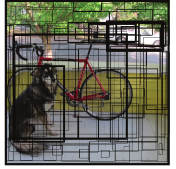
\includegraphics[width=9cm,height=9cm,keepaspectratio]{focal_loss.png}
	\caption{Ví dụ về sự mất cân bằng giữa  foreground và background\cite{lin2018focal}}
	\label{fig:focal_loss}
\end{figure}
\bigskip
{\fontsize{13}{12} \selectfont

	RetinaNet là sự kết hợp giữa các mạng bao gồm backbone và mạng con. Dữ
	liệu đầu vào của RetinaNet được đưa qua mô hình mạng có tên là FPN \cite{lin2017feature} nhằm rút trích các ma trận đặc trưng với
	cùng một tỉ lệ nhưng theo nhiều kích thước khác nhau. Sau đó từ ma trận đặc trưng mới bắt đầu tính toán các vùng để
	xuất. Cuối cùng các vùng đề xuất được đưa qua hai mạng phụ để tính ra vị trí của các hộp giới và lớp của đối
	tượng mà hộp đó bao quanh. Hình \ref{fig:retinanet} mô tả kiến trúc của Retinanet gồm hai phần. Phần backbone là
	là một trích xuất đặc trưng kết hợp giữa Resnet + FPN. Phần mạng con dùng để phân lớp và
	xác định vị trí hộp giới hạn.
}

\begin{figure}[H]
	\centering
	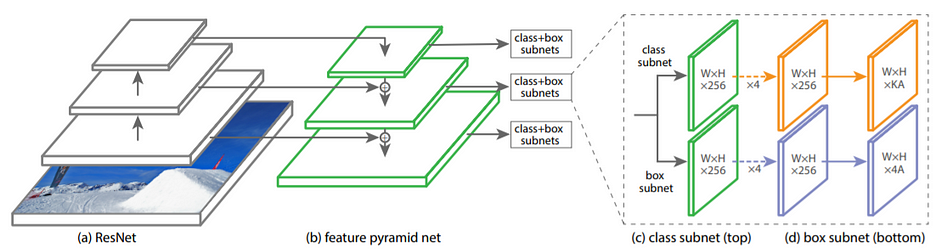
\includegraphics[width=1\textwidth]{retinanet.png}
	\caption{Cấu trúc mạng Retinanet \cite{lin2018focal}}
	\label{fig:retinanet}
\end{figure}
\bigskip


\section{Các phương pháp đánh giá mô hình}
\subsection{Phương pháp đánh giá IoU (Intersection over Union)}
{\fontsize{13}{12} \selectfont
	IoU là chỉ số đánh giá các mô hình phát hiện vật thể. IoU là tỉ lệ giữa vùng giao và hợp của kết quả dự đoán và kết quả thực tế (Hình \ref{fig:iou}).
	Giá trị của IoU dao động
	từ 0 đến 1, với 0 nghĩa là không có sự chồng chéo giữa kết quả dự đoán và kết quả
	thực tế và 1 nghĩa là hai kết quả này hoàn toàn trùng khớp
	Tỉ lệ này càng lớn đồng nghĩa hôp giới hạn dự đoán ra càng giống hộp thực của dữ liệu.
}

\begin{figure}[H]
	\centering
	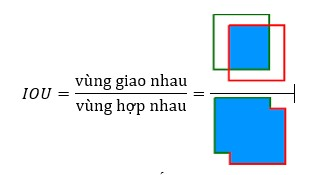
\includegraphics[width=1\textwidth]{iou.jpg}
	\caption{Chỉ số đánh giá IoU}
	\label{fig:iou}
\end{figure}
\bigskip

{\fontsize{13}{12} \selectfont
	Trong hình \ref{fig:iou} có khung màu đỏ là nhãn thực hay còn gọi là hộp giới hạn
	được gán nhãn, khung màu xanh là nhãn dự đoán hay còn gọi là hộp giới hạn được mô hình dự đoán.
	Kết quả của Iou sẽ có giá trị trong khoảng 0 đến 1 với mỗi lần phát hiện có giá trị riêng. Để xác định là phát hiện đúng hoặc phát hiện sai, chúng ta phải dựa vào ngưỡng cho trước.
	Thông thường với các mô hình phát hiện đôi tượng, chỉ số $IoU > 50\%$ được xem là dự đoán có đối tượng. Dựa vào khái niệm trên ta có các định nghĩa sau:
	\begin{itemize}
		\item True Positive (TP): IoU lớn hơn hoặc bằng ngưỡng, là một dự đoán đúng.
		\item False Positive (FP): IoU bé hơn ngưỡng, là một dự đoán sai.
		\item False Negative (FN): trường hợp mà hộp giới hạn đúng nhưng không có hộp dự đoán.
	\end{itemize}
}

\subsection{Phương pháp đánh giá độ chính xác, độ nhạy, độ chính xác trung bình}
{\fontsize{13}{12} \selectfont
	Độ chính xác (precision) đo lường tỷ lệ các dự đoán tích cực mà hệ thống phân loại đưa ra
	mà thực tế là đúng có công thức \ref{equa:P}.
	Độ nhạy (recall) đo lường tỷ lệ của các hộp giới hạn mà mô hình dự đoán đúng so với tổng số các hộp giới hạn dữ liệu thực tế đúng có công thức \ref{equa:R}.
	Giá tri TP của mô hình sẽ phụ thuộc vào việc chọn ngưỡng IoU.
	Như hình \ref{fig:nguong_iou} nếu ngưỡng IoU là 0.5, IoU cho dự đoán là 0.7 khi đó chúng ta có TP - dự đoán đúng. Ngược lại nếu IoU là 0.3, chúng ta có FP - dự đoán sai.
	\begin{equation}
		Precision = \frac{TP}{TP+FP}\
		\label{equa:P}
	\end{equation}
	\begin{equation}
		Precision = \frac{TP}{TP+FN}\
		\label{equa:R}
	\end{equation}
}
\begin{figure}[H]
	\centering
	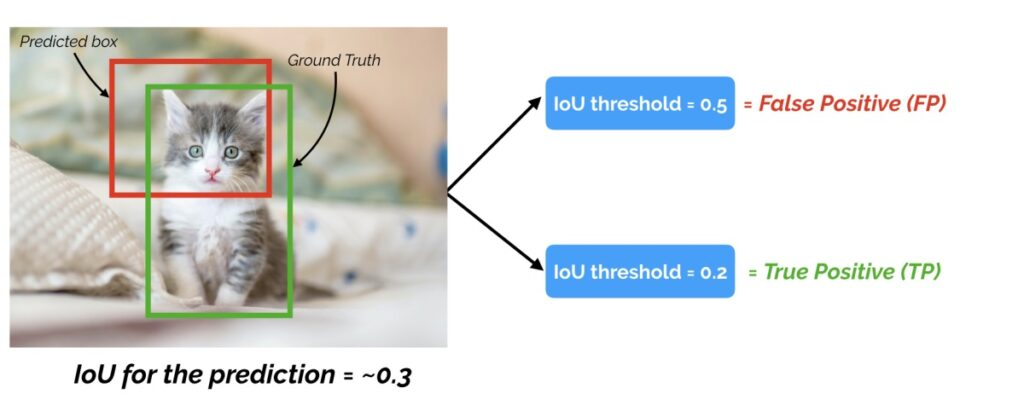
\includegraphics[width=1\textwidth]{nguong_iou.jpg}
	\caption{Ví dụ về việc thay đổi ngưỡng IoU}
	\label{fig:nguong_iou}
\end{figure}
\bigskip

{\fontsize{13}{12} \selectfont
	Khi bắt đầu thay đổi ngưỡng IoU, các giá trị precision và recall sẽ được tính để tạo ra đường cong được gọi là Precision Recall Curve tương tự hình \ref{fig:ap}.
	Chỉ số độ chính xác trung bình - Average Precision (AP) là diện tích vùng màu xanh ở hình \ref{fig:ap}. AP càng lớn thể hiện việc precision và recall càng cao với các ngưỡng IoU khác nhau, đồng nghĩa với mô hình tốt.

	mAP (mean average precision) là trung bình của AP. Trong một số trường hợp chúng ta tính AP cho mỗi lớp và lấy trung bình. Nhưng trong một số trường hợp khác AP và mAP lại giống nhau phụ thuộc vào từng bài toán.
	Trong PASCAL VOC2007, AP cho một lớp được tính cho một ngưỡng IoU. Do đó mAP là trung bình của AP trên toàn bộ các lớp.
	Còn trong COCO 2017, mAP là trung bình trên toàn bộ các lớp và với mười ngưỡng IoU.
}
\begin{figure}[H]
	\centering
	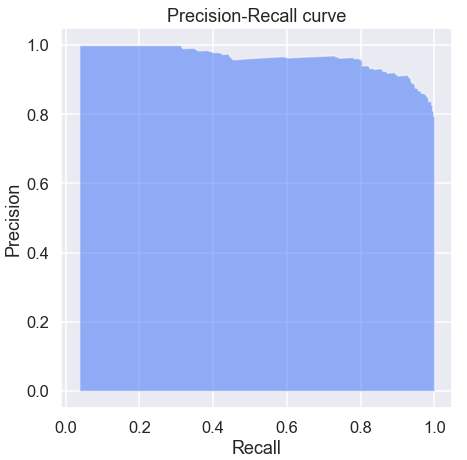
\includegraphics[width=1\textwidth]{AP.png}
	\caption{Precision Recall Curve được vẽ với ngưỡng IoU chạy từ 0 đến 1}
	\label{fig:ap}
\end{figure}
\subsection{Phương pháp đánh giá bằng tốc độ, thông số, độ lớn của mô hình}
{\fontsize{13}{12} \selectfont
	Khung hình trên giây (FPS) biểu thị số lượng khung hình mà mô hình phát hiện đối tượng có thể xử lý mỗi giây. Nó là thước đo tốc độ và hiệu quả của mô hình, cho biết mô hình có thể xử lý các hình ảnh đến và tạo ra kết quả phát hiện đối tượng nhanh như thế nào.
	Với việc mở rộng phát triển mô hình sau này của bài toán, việc chọn FPS cao sẽ giúp cải thiện trải nghiệm người dùng và thuận tiện cho việc xử lí thời gian thực.

	Thông số cho biết số lượng tham số có thể học được trong một mô hình. Đó là thước đo độ phức tạp của mô hình và dung lượng bộ nhớ. Việc phát hiện rác cần các dữ liệu bổ sung để cải thiện độ chính xác của mô hình, vì vậy việc tiếp tục huấn luyện dựa trên các hình ảnh được người dùng cung cấp là rất quan trọng.
	Thời gian huấn luyện mô hình nhanh dựa vào các tham số trong mô hình giúp việc cải thiện hệ thống nhanh hơn.

	Kích thước thể hiện kích thước tệp hoặc mức tiêu thụ bộ nhớ của mô hình. Nó đo lường tính di động của mô hình và khả năng triển khai dễ dàng.
	kích thước nhỏ hơn sẽ dễ dàng lưu trữ và truyền tải hơn, yêu cầu tài nguyên trên thiết bị thấp hơn, có khả năng tải xuống và triển khai nhanh hơn. Hệ thống hướng tới việc triển khai trên thiết bị di động nên việc chọn các mô hình có kích thước nhỏ là việc ưu tiên.
}
% \begin{algorithm}
% \caption{Thuật toán NMS}\label{alg:1}
% \begin{algorithmic}
% \KwData{$n \geq 0$}
% \KwResult{$y = x^n$}
% \State $y \gets 1$
% \State $X \gets x$
% \State $N \gets n$
% \While{$N \neq 0$}
% \If{$N$ is even}
%     \State $X \gets X \times X$
%     \State $N \gets \frac{N}{2}$  \Comment{This is a comment}
% \ElsIf{$N$ is odd}
%     \State $y \gets y \times X$
%     \State $N \gets N - 1$
% \EndIf
% \EndWhile
% \end{algorithmic}
% \end{algorithm}
\end{document}